% Options for packages loaded elsewhere
\PassOptionsToPackage{unicode}{hyperref}
\PassOptionsToPackage{hyphens}{url}
%
\documentclass[
]{article}
\usepackage{lmodern}
\usepackage{amssymb,amsmath}
\usepackage{ifxetex,ifluatex}
\ifnum 0\ifxetex 1\fi\ifluatex 1\fi=0 % if pdftex
  \usepackage[T1]{fontenc}
  \usepackage[utf8]{inputenc}
  \usepackage{textcomp} % provide euro and other symbols
\else % if luatex or xetex
  \usepackage{unicode-math}
  \defaultfontfeatures{Scale=MatchLowercase}
  \defaultfontfeatures[\rmfamily]{Ligatures=TeX,Scale=1}
\fi
% Use upquote if available, for straight quotes in verbatim environments
\IfFileExists{upquote.sty}{\usepackage{upquote}}{}
\IfFileExists{microtype.sty}{% use microtype if available
  \usepackage[]{microtype}
  \UseMicrotypeSet[protrusion]{basicmath} % disable protrusion for tt fonts
}{}
\makeatletter
\@ifundefined{KOMAClassName}{% if non-KOMA class
  \IfFileExists{parskip.sty}{%
    \usepackage{parskip}
  }{% else
    \setlength{\parindent}{0pt}
    \setlength{\parskip}{6pt plus 2pt minus 1pt}}
}{% if KOMA class
  \KOMAoptions{parskip=half}}
\makeatother
\usepackage{xcolor}
\IfFileExists{xurl.sty}{\usepackage{xurl}}{} % add URL line breaks if available
\IfFileExists{bookmark.sty}{\usepackage{bookmark}}{\usepackage{hyperref}}
\hypersetup{
  pdftitle={Organoid Unsupervised Exploration},
  pdfauthor={Niklas Rindtorff},
  hidelinks,
  pdfcreator={LaTeX via pandoc}}
\urlstyle{same} % disable monospaced font for URLs
\usepackage[margin=1in]{geometry}
\usepackage{color}
\usepackage{fancyvrb}
\newcommand{\VerbBar}{|}
\newcommand{\VERB}{\Verb[commandchars=\\\{\}]}
\DefineVerbatimEnvironment{Highlighting}{Verbatim}{commandchars=\\\{\}}
% Add ',fontsize=\small' for more characters per line
\usepackage{framed}
\definecolor{shadecolor}{RGB}{248,248,248}
\newenvironment{Shaded}{\begin{snugshade}}{\end{snugshade}}
\newcommand{\AlertTok}[1]{\textcolor[rgb]{0.94,0.16,0.16}{#1}}
\newcommand{\AnnotationTok}[1]{\textcolor[rgb]{0.56,0.35,0.01}{\textbf{\textit{#1}}}}
\newcommand{\AttributeTok}[1]{\textcolor[rgb]{0.77,0.63,0.00}{#1}}
\newcommand{\BaseNTok}[1]{\textcolor[rgb]{0.00,0.00,0.81}{#1}}
\newcommand{\BuiltInTok}[1]{#1}
\newcommand{\CharTok}[1]{\textcolor[rgb]{0.31,0.60,0.02}{#1}}
\newcommand{\CommentTok}[1]{\textcolor[rgb]{0.56,0.35,0.01}{\textit{#1}}}
\newcommand{\CommentVarTok}[1]{\textcolor[rgb]{0.56,0.35,0.01}{\textbf{\textit{#1}}}}
\newcommand{\ConstantTok}[1]{\textcolor[rgb]{0.00,0.00,0.00}{#1}}
\newcommand{\ControlFlowTok}[1]{\textcolor[rgb]{0.13,0.29,0.53}{\textbf{#1}}}
\newcommand{\DataTypeTok}[1]{\textcolor[rgb]{0.13,0.29,0.53}{#1}}
\newcommand{\DecValTok}[1]{\textcolor[rgb]{0.00,0.00,0.81}{#1}}
\newcommand{\DocumentationTok}[1]{\textcolor[rgb]{0.56,0.35,0.01}{\textbf{\textit{#1}}}}
\newcommand{\ErrorTok}[1]{\textcolor[rgb]{0.64,0.00,0.00}{\textbf{#1}}}
\newcommand{\ExtensionTok}[1]{#1}
\newcommand{\FloatTok}[1]{\textcolor[rgb]{0.00,0.00,0.81}{#1}}
\newcommand{\FunctionTok}[1]{\textcolor[rgb]{0.00,0.00,0.00}{#1}}
\newcommand{\ImportTok}[1]{#1}
\newcommand{\InformationTok}[1]{\textcolor[rgb]{0.56,0.35,0.01}{\textbf{\textit{#1}}}}
\newcommand{\KeywordTok}[1]{\textcolor[rgb]{0.13,0.29,0.53}{\textbf{#1}}}
\newcommand{\NormalTok}[1]{#1}
\newcommand{\OperatorTok}[1]{\textcolor[rgb]{0.81,0.36,0.00}{\textbf{#1}}}
\newcommand{\OtherTok}[1]{\textcolor[rgb]{0.56,0.35,0.01}{#1}}
\newcommand{\PreprocessorTok}[1]{\textcolor[rgb]{0.56,0.35,0.01}{\textit{#1}}}
\newcommand{\RegionMarkerTok}[1]{#1}
\newcommand{\SpecialCharTok}[1]{\textcolor[rgb]{0.00,0.00,0.00}{#1}}
\newcommand{\SpecialStringTok}[1]{\textcolor[rgb]{0.31,0.60,0.02}{#1}}
\newcommand{\StringTok}[1]{\textcolor[rgb]{0.31,0.60,0.02}{#1}}
\newcommand{\VariableTok}[1]{\textcolor[rgb]{0.00,0.00,0.00}{#1}}
\newcommand{\VerbatimStringTok}[1]{\textcolor[rgb]{0.31,0.60,0.02}{#1}}
\newcommand{\WarningTok}[1]{\textcolor[rgb]{0.56,0.35,0.01}{\textbf{\textit{#1}}}}
\usepackage{graphicx,grffile}
\makeatletter
\def\maxwidth{\ifdim\Gin@nat@width>\linewidth\linewidth\else\Gin@nat@width\fi}
\def\maxheight{\ifdim\Gin@nat@height>\textheight\textheight\else\Gin@nat@height\fi}
\makeatother
% Scale images if necessary, so that they will not overflow the page
% margins by default, and it is still possible to overwrite the defaults
% using explicit options in \includegraphics[width, height, ...]{}
\setkeys{Gin}{width=\maxwidth,height=\maxheight,keepaspectratio}
% Set default figure placement to htbp
\makeatletter
\def\fps@figure{htbp}
\makeatother
\setlength{\emergencystretch}{3em} % prevent overfull lines
\providecommand{\tightlist}{%
  \setlength{\itemsep}{0pt}\setlength{\parskip}{0pt}}
\setcounter{secnumdepth}{-\maxdimen} % remove section numbering

\title{Organoid Unsupervised Exploration}
\author{Niklas Rindtorff}
\date{}

\begin{document}
\maketitle

Loading packages

\begin{Shaded}
\begin{Highlighting}[]
\KeywordTok{library}\NormalTok{(ggplot2)}
\KeywordTok{library}\NormalTok{(dplyr)}
\KeywordTok{library}\NormalTok{(tidyr)}
\KeywordTok{library}\NormalTok{(magrittr)}
\KeywordTok{library}\NormalTok{(purrr)}
\KeywordTok{library}\NormalTok{(readr)}
\KeywordTok{library}\NormalTok{(here)}
\KeywordTok{library}\NormalTok{(ggrastr)}
\KeywordTok{library}\NormalTok{(cowplot)}
\KeywordTok{library}\NormalTok{(princurve)}
\KeywordTok{library}\NormalTok{(scico)}
\KeywordTok{library}\NormalTok{(ggridges)}

\CommentTok{# parameter}
\KeywordTok{print}\NormalTok{(}\StringTok{"parameter input:"}\NormalTok{)}
\end{Highlighting}
\end{Shaded}

\begin{verbatim}
## [1] "parameter input:"
\end{verbatim}

\begin{Shaded}
\begin{Highlighting}[]
\KeywordTok{print}\NormalTok{(params}\OperatorTok{$}\NormalTok{data)}
\end{Highlighting}
\end{Shaded}

\begin{verbatim}
## [1] "data/processed/PhenotypeSpectrum/umap_absolute_all_drugs_sampled.Rds"
\end{verbatim}

\begin{Shaded}
\begin{Highlighting}[]
\KeywordTok{print}\NormalTok{(params}\OperatorTok{$}\NormalTok{sample)}
\end{Highlighting}
\end{Shaded}

\begin{verbatim}
## [1] "data/processed/PhenotypeSpectrum/umap_absolute_all_drugs_tidy_Paclitaxel.Rds"
\end{verbatim}

loading input data and annotation. Note that on the central cluster,
with access to the complete data table, the definition of the input can
easily be changed. For remote work, the subsampled dataset
``umap\_drugs\_sampled.Rds'' is the default choice.

\begin{Shaded}
\begin{Highlighting}[]
\CommentTok{# I wish I could solve my path problems with the here() package, but experienced unreliable behavior }
\CommentTok{# PATH = "/dkfz/groups/shared/OE0049/B110-Isilon2/promise/"}
\NormalTok{PATH =}\StringTok{ }\KeywordTok{paste0}\NormalTok{(here}\OperatorTok{::}\KeywordTok{here}\NormalTok{(), }\StringTok{"/"}\NormalTok{)}

\CommentTok{#umap_df <- read_rds(paste0(PATH, "data/processed/PhenotypeSpectrum/umap_absolute_all_drugs_tidy.Rds"))}
\CommentTok{#umap_df <- read_rds(paste0(PATH, "data/processed/PhenotypeSpectrum/umap_absolute_all_drugs_sampled.Rds"))}
\NormalTok{umap_df <-}\StringTok{ }\KeywordTok{read_rds}\NormalTok{(here}\OperatorTok{::}\KeywordTok{here}\NormalTok{(params}\OperatorTok{$}\NormalTok{data))}
\NormalTok{umap_df_sample <-}\StringTok{ }\KeywordTok{read_rds}\NormalTok{(here}\OperatorTok{::}\KeywordTok{here}\NormalTok{(params}\OperatorTok{$}\NormalTok{sample))}

\NormalTok{organoid_morphology <-}\StringTok{ }\KeywordTok{read_delim}\NormalTok{(here}\OperatorTok{::}\KeywordTok{here}\NormalTok{(}\StringTok{"references/imaging/visual_classification_organoids.csv"}\NormalTok{), }\StringTok{";"}\NormalTok{, }\DataTypeTok{escape_double =} \OtherTok{FALSE}\NormalTok{, }\DataTypeTok{trim_ws =} \OtherTok{TRUE}\NormalTok{) }\OperatorTok\StringTok{ }
\StringTok{  }\NormalTok{dplyr}\OperatorTok{::}\KeywordTok{select}\NormalTok{(}\DataTypeTok{line =}\NormalTok{ organoid, }\DataTypeTok{morphology =}\NormalTok{ visual_inspection_v2)}

\CommentTok{#organoid_viability <- read_rds(here::here("data/processed/ldc_viability.rds"))}
\end{Highlighting}
\end{Shaded}

\hypertarget{data-cube}{%
\section{Data cube}\label{data-cube}}

\begin{Shaded}
\begin{Highlighting}[]
\NormalTok{umap_df }\OperatorTok\StringTok{ }\NormalTok{dplyr}\OperatorTok{::}\KeywordTok{distinct}\NormalTok{(drug, line) }\OperatorTok\StringTok{ }\NormalTok{dplyr}\OperatorTok{::}\KeywordTok{count}\NormalTok{(line)}
\end{Highlighting}
\end{Shaded}

\begin{verbatim}
## # A tibble: 12 x 2
##    line        n
##    <chr>   <int>
##  1 D004T01   528
##  2 D007T01   528
##  3 D010T01   528
##  4 D013T01   528
##  5 D018T01   528
##  6 D019T01   528
##  7 D020T01   528
##  8 D020T02   528
##  9 D022T01   528
## 10 D027T01   528
## 11 D030T01   528
## 12 D046T01   528
\end{verbatim}

\hypertarget{partition-inspection}{%
\section{Partition inspection}\label{partition-inspection}}

We are able to observe 4 partitions in our data. After manual
inspection, it becomes cleat that the two smallest partitions are mostly
consisting of

\begin{Shaded}
\begin{Highlighting}[]
\NormalTok{umap_df }\OperatorTok\StringTok{ }
\StringTok{  }\KeywordTok{ggplot}\NormalTok{(}\KeywordTok{aes}\NormalTok{(v1, v2, }\DataTypeTok{color =} \KeywordTok{factor}\NormalTok{(partition))) }\OperatorTok{+}\StringTok{ }
\StringTok{  }\KeywordTok{geom_point_rast}\NormalTok{(}\DataTypeTok{alpha =} \FloatTok{0.5}\NormalTok{, }\DataTypeTok{size =} \FloatTok{0.35}\NormalTok{) }\OperatorTok{+}\StringTok{ }
\StringTok{  }\KeywordTok{scale_color_brewer}\NormalTok{(}\DataTypeTok{type =} \StringTok{"qual"}\NormalTok{, }\DataTypeTok{palette =} \StringTok{"Set2"}\NormalTok{) }\OperatorTok{+}
\StringTok{  }\KeywordTok{theme_cowplot}\NormalTok{() }\OperatorTok{+}
\StringTok{  }\KeywordTok{labs}\NormalTok{(}\DataTypeTok{x =} \StringTok{"UMAP 1"}\NormalTok{,}
       \DataTypeTok{y =} \StringTok{"UMAP 2"}\NormalTok{,}
       \DataTypeTok{color =} \StringTok{"partition"}\NormalTok{) }\OperatorTok{+}\StringTok{ }
\StringTok{  }\KeywordTok{theme}\NormalTok{(}\DataTypeTok{legend.position =} \StringTok{"bottom"}\NormalTok{) }\OperatorTok{+}\StringTok{ }
\StringTok{    }\KeywordTok{coord_fixed}\NormalTok{()}
\end{Highlighting}
\end{Shaded}

\includegraphics{organoid_unsupervised_exploration_files/figure-latex/unnamed-chunk-4-1.pdf}

\begin{Shaded}
\begin{Highlighting}[]
\NormalTok{umap_df }\OperatorTok\StringTok{ }
\StringTok{  }\NormalTok{dplyr}\OperatorTok{::}\KeywordTok{count}\NormalTok{(partition) }\OperatorTok\StringTok{ }
\StringTok{  }\KeywordTok{mutate}\NormalTok{(}\DataTypeTok{ratio =}\NormalTok{ n}\OperatorTok{/}\KeywordTok{sum}\NormalTok{(n)) }\OperatorTok\StringTok{ }
\StringTok{  }\KeywordTok{arrange}\NormalTok{(}\KeywordTok{desc}\NormalTok{(ratio))}
\end{Highlighting}
\end{Shaded}

\begin{verbatim}
## # A tibble: 1 x 3
##   partition      n ratio
##   <fct>      <int> <dbl>
## 1 1         271308     1
\end{verbatim}

I remove 2 partitions from all main figures for ease of reading. Below,
it is easy to toggle the removal of partitions on and off to make sure
this filtering step is robust

\begin{Shaded}
\begin{Highlighting}[]
\NormalTok{gg_cluster <-}\StringTok{ }\NormalTok{umap_df }\OperatorTok
\StringTok{  }\KeywordTok{filter}\NormalTok{(partition }\OperatorTok\StringTok{ }\KeywordTok{c}\NormalTok{(}\DecValTok{1}\NormalTok{,}\DecValTok{2}\NormalTok{)) }\OperatorTok
\StringTok{  }\KeywordTok{ggplot}\NormalTok{(}\KeywordTok{aes}\NormalTok{(v1, v2, }\DataTypeTok{color =} \KeywordTok{factor}\NormalTok{(cluster))) }\OperatorTok{+}\StringTok{ }
\StringTok{  }\NormalTok{ggrastr}\OperatorTok{::}\KeywordTok{geom_point_rast}\NormalTok{(}\DataTypeTok{alpha =} \FloatTok{0.5}\NormalTok{, }\DataTypeTok{size =} \FloatTok{0.35}\NormalTok{) }\OperatorTok{+}\StringTok{ }
\StringTok{  }\KeywordTok{scale_color_manual}\NormalTok{(}\DataTypeTok{values =} \KeywordTok{c}\NormalTok{(RColorBrewer}\OperatorTok{::}\KeywordTok{brewer.pal}\NormalTok{(}\DecValTok{12}\NormalTok{, }\StringTok{"Set3"}\NormalTok{), }\StringTok{"#fb9a99"}\NormalTok{)) }\OperatorTok{+}
\StringTok{  }\NormalTok{cowplot}\OperatorTok{::}\KeywordTok{theme_cowplot}\NormalTok{() }\OperatorTok{+}
\StringTok{  }\KeywordTok{labs}\NormalTok{(}\DataTypeTok{x =} \StringTok{"UMAP 1"}\NormalTok{,}
       \DataTypeTok{y =} \StringTok{"UMAP 2"}\NormalTok{,}
       \DataTypeTok{color =} \StringTok{"partition"}\NormalTok{) }\OperatorTok{+}\StringTok{ }
\StringTok{  }\KeywordTok{theme}\NormalTok{(}\DataTypeTok{legend.position =} \StringTok{"bottom"}\NormalTok{) }\OperatorTok{+}\StringTok{ }
\StringTok{    }\KeywordTok{coord_fixed}\NormalTok{()}

\NormalTok{gg_cluster }\OperatorTok{+}\StringTok{ }\KeywordTok{ggsave}\NormalTok{(}\KeywordTok{here}\NormalTok{(}\StringTok{"reports/figures/imaging/gg_cluster.pdf"}\NormalTok{), }\DataTypeTok{width =} \DecValTok{4}\NormalTok{, }\DataTypeTok{height =} \DecValTok{4}\NormalTok{)}
\end{Highlighting}
\end{Shaded}

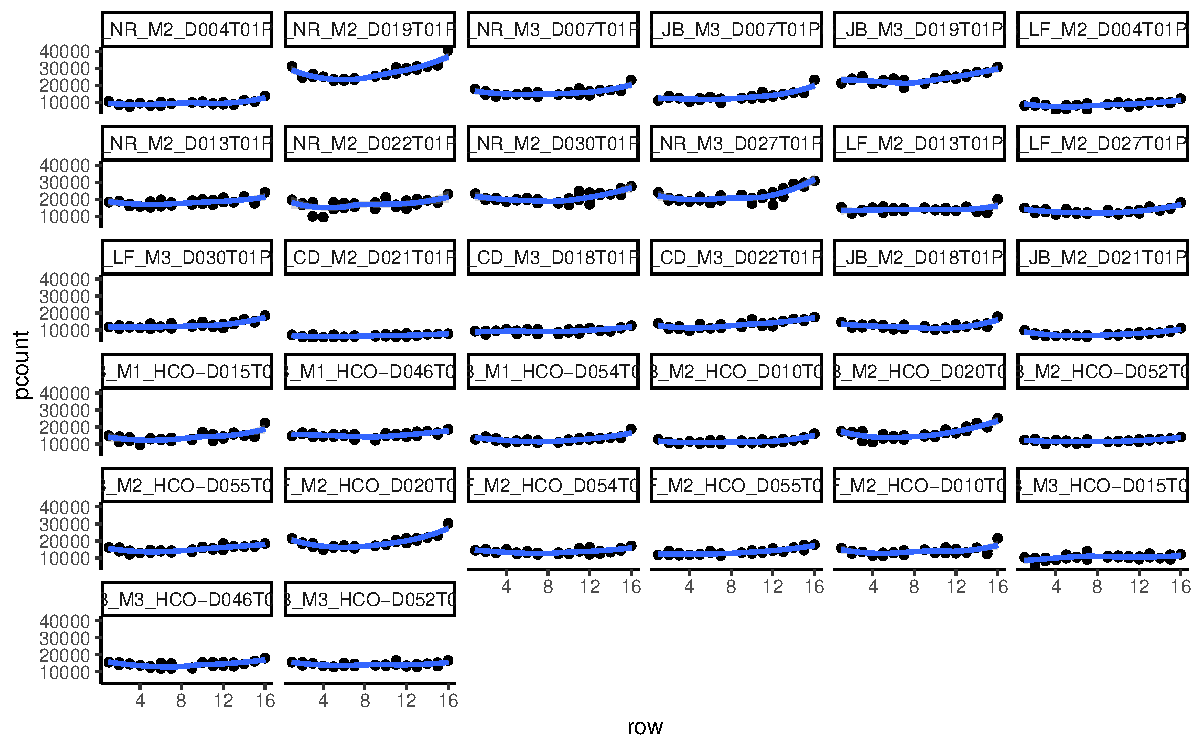
\includegraphics{organoid_unsupervised_exploration_files/figure-latex/unnamed-chunk-6-1.pdf}

\hypertarget{organoid-size-distributions}{%
\section{Organoid Size
Distributions}\label{organoid-size-distributions}}

I plot a size-distribution.

\begin{Shaded}
\begin{Highlighting}[]
\NormalTok{gg_size_dist <-}\StringTok{ }\NormalTok{umap_df }\OperatorTok\StringTok{ }
\StringTok{  }\KeywordTok{filter}\NormalTok{(partition }\OperatorTok\StringTok{ }\KeywordTok{c}\NormalTok{(}\DecValTok{1}\NormalTok{,}\DecValTok{2}\NormalTok{)) }\OperatorTok
\StringTok{  }\KeywordTok{ggplot}\NormalTok{(}\KeywordTok{aes}\NormalTok{(size)) }\OperatorTok{+}\StringTok{ }
\StringTok{  }\KeywordTok{geom_histogram}\NormalTok{() }\OperatorTok{+}\StringTok{ }
\StringTok{  }\KeywordTok{theme_cowplot}\NormalTok{() }\OperatorTok{+}\StringTok{ }
\StringTok{  }\KeywordTok{labs}\NormalTok{(}\DataTypeTok{caption =} \StringTok{"all treatments, downsampled"}\NormalTok{)}

\NormalTok{gg_size_dist_log <-}\StringTok{ }\NormalTok{gg_size_dist }\OperatorTok{+}\StringTok{ }
\StringTok{  }\KeywordTok{scale_x_log10}\NormalTok{()}

\NormalTok{gg_size_dist_log }\OperatorTok{+}\StringTok{ }\KeywordTok{ggsave}\NormalTok{(}\KeywordTok{here}\NormalTok{(}\StringTok{"reports/figures/imaging/gg_size_dist.pdf"}\NormalTok{), }\DataTypeTok{width =} \DecValTok{4}\NormalTok{, }\DataTypeTok{height =} \DecValTok{4}\NormalTok{)}
\end{Highlighting}
\end{Shaded}

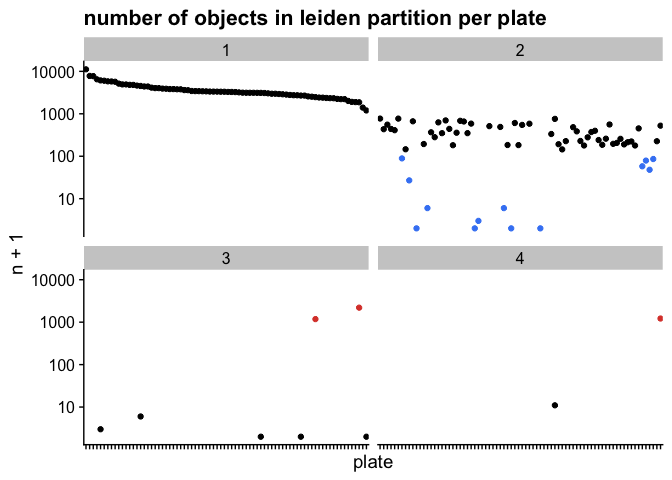
\includegraphics{organoid_unsupervised_exploration_files/figure-latex/unnamed-chunk-7-1.pdf}

I add the eCDF.

\begin{Shaded}
\begin{Highlighting}[]
\NormalTok{df <-}\StringTok{ }\NormalTok{umap_df }\OperatorTok\StringTok{ }\KeywordTok{filter}\NormalTok{(partition }\OperatorTok\StringTok{ }\KeywordTok{c}\NormalTok{(}\DecValTok{1}\NormalTok{,}\DecValTok{2}\NormalTok{))}

\NormalTok{gg_ecdf <-}\StringTok{ }\KeywordTok{ggplot}\NormalTok{(df }\OperatorTok\StringTok{ }\KeywordTok{filter}\NormalTok{(drug }\OperatorTok{==}\StringTok{ "DMSO"}\NormalTok{)) }\OperatorTok{+}
\StringTok{  }\KeywordTok{stat_ecdf}\NormalTok{(}\KeywordTok{aes}\NormalTok{(}\DataTypeTok{x =}\NormalTok{ size, }\DataTypeTok{group =}\NormalTok{ line), }
              \DataTypeTok{geom =} \StringTok{"step"}\NormalTok{, }\DataTypeTok{size =} \DecValTok{1}\NormalTok{) }\OperatorTok{+}
\StringTok{  }\CommentTok{#scale_color_manual(values = c("#00AFBB", "#E7B800"))+}
\StringTok{  }\KeywordTok{labs}\NormalTok{(}\DataTypeTok{y =} \StringTok{"f(size)"}\NormalTok{,}
       \DataTypeTok{x =} \StringTok{"organoid size [pixels]"}\NormalTok{) }\OperatorTok{+}\StringTok{ }
\StringTok{  }\KeywordTok{theme_cowplot}\NormalTok{()}

\NormalTok{gg_ecdf}
\end{Highlighting}
\end{Shaded}

\includegraphics{organoid_unsupervised_exploration_files/figure-latex/unnamed-chunk-8-1.pdf}

\begin{Shaded}
\begin{Highlighting}[]
\CommentTok{# variance_explained %>% ggplot(aes(PC, var_explained)) + geom_point() + geom_vline(xintercept = 25) + scale_y_sqrt()}


\CommentTok{# element wise multiplication}
\NormalTok{mat =}\StringTok{ }\NormalTok{components }\OperatorTok\StringTok{ }\NormalTok{dplyr}\OperatorTok{::}\KeywordTok{select}\NormalTok{(}\OperatorTok{-}\NormalTok{X1) }\OperatorTok\StringTok{ }\KeywordTok{as.matrix}\NormalTok{() }\OperatorTok\StringTok{ }\NormalTok{.[,}\DecValTok{1}\OperatorTok{:}\DecValTok{25}\NormalTok{] }\OperatorTok\StringTok{ }\KeywordTok{matrix}\NormalTok{(}\DataTypeTok{ncol =} \DecValTok{25}\NormalTok{)}
\NormalTok{vector =}\StringTok{ }\KeywordTok{sqrt}\NormalTok{(variance_explained}\OperatorTok{$}\NormalTok{eigenvalue) }\OperatorTok\StringTok{ }\NormalTok{.[}\DecValTok{1}\OperatorTok{:}\DecValTok{25}\NormalTok{]}
\NormalTok{df =}\StringTok{ }\NormalTok{mat }\OperatorTok{*}\StringTok{ }\NormalTok{vector}

\NormalTok{index =}\StringTok{ }\NormalTok{df }\OperatorTok\StringTok{ }\KeywordTok{abs}\NormalTok{() }\OperatorTok\StringTok{ }\KeywordTok{rowSums}\NormalTok{() }\OperatorTok\StringTok{ }\KeywordTok{tibble}\NormalTok{(}\DataTypeTok{max =}\NormalTok{ ., }\DataTypeTok{index =} \DecValTok{1}\OperatorTok{:}\KeywordTok{length}\NormalTok{(.)) }\OperatorTok\StringTok{ }\KeywordTok{arrange}\NormalTok{(}\KeywordTok{desc}\NormalTok{(max)) }\OperatorTok\StringTok{ }\KeywordTok{head}\NormalTok{(}\DecValTok{25}\NormalTok{) }\OperatorTok\StringTok{ }\NormalTok{.}\OperatorTok{$}\NormalTok{index}

\NormalTok{pheatmap}\OperatorTok{::}\KeywordTok{pheatmap}\NormalTok{(}\DataTypeTok{mat =}\NormalTok{ annotated_PC }\OperatorTok\StringTok{ }\NormalTok{dplyr}\OperatorTok{::}\KeywordTok{select}\NormalTok{(name, PC1}\OperatorTok{:}\NormalTok{PC25) }\OperatorTok\StringTok{ }\NormalTok{.[index,] }\OperatorTok\StringTok{ }\KeywordTok{remove_rownames}\NormalTok{() }\OperatorTok\StringTok{  }\NormalTok{tibble}\OperatorTok{::}\KeywordTok{column_to_rownames}\NormalTok{(}\StringTok{'name'}\NormalTok{),}
                   \DataTypeTok{annotation_row =}\NormalTok{ annotated_PC }\OperatorTok\StringTok{ }\NormalTok{dplyr}\OperatorTok{::}\KeywordTok{select}\NormalTok{(name, class, channel) }\OperatorTok\StringTok{ }\NormalTok{.[index,] }\OperatorTok\StringTok{ }\NormalTok{tibble}\OperatorTok{::}\KeywordTok{column_to_rownames}\NormalTok{(}\StringTok{'name'}\NormalTok{),}
                   \DataTypeTok{cluster_cols =} \OtherTok{FALSE}\NormalTok{)}
\end{Highlighting}
\end{Shaded}

For more details about distributions, please refer to
*reports/Phenotypespectrum/`xyz'\_dist.pdf*.

\begin{Shaded}
\begin{Highlighting}[]
\NormalTok{line_param <-}\StringTok{ }\NormalTok{umap_df }\OperatorTok\StringTok{ }\KeywordTok{filter}\NormalTok{(partition }\OperatorTok\StringTok{ }\KeywordTok{c}\NormalTok{(}\DecValTok{1}\NormalTok{,}\DecValTok{2}\NormalTok{)) }\OperatorTok\StringTok{ }
\StringTok{  }\CommentTok{#filter(drug == "DMSO") %>%}
\StringTok{  }\KeywordTok{nest}\NormalTok{(}\OperatorTok{-}\NormalTok{line, }\OperatorTok{-}\NormalTok{replicate) }\OperatorTok\StringTok{ }
\StringTok{  }\KeywordTok{mutate}\NormalTok{(}\DataTypeTok{fit =} \KeywordTok{map}\NormalTok{(data, }\OperatorTok{~}\StringTok{ }\NormalTok{fitdistrplus}\OperatorTok{::}\KeywordTok{fitdist}\NormalTok{(.x}\OperatorTok{$}\NormalTok{size, }\StringTok{"lnorm"}\NormalTok{)),}
         \DataTypeTok{param =} \KeywordTok{map}\NormalTok{(fit, }\OperatorTok{~}\StringTok{ }\NormalTok{.x}\OperatorTok{$}\NormalTok{estimate }\OperatorTok\StringTok{ }\NormalTok{broom}\OperatorTok{::}\KeywordTok{tidy}\NormalTok{()))}

\NormalTok{df <-}\StringTok{ }\NormalTok{line_param }\OperatorTok\StringTok{ }\KeywordTok{unnest}\NormalTok{(param) }\OperatorTok\StringTok{ }
\StringTok{  }\KeywordTok{filter}\NormalTok{(names }\OperatorTok{==}\StringTok{ "meanlog"}\NormalTok{) }\OperatorTok\StringTok{ }
\StringTok{  }\KeywordTok{group_by}\NormalTok{(line) }\OperatorTok\StringTok{ }
\StringTok{  }\KeywordTok{mutate}\NormalTok{(}\DataTypeTok{mean_meanlog =} \KeywordTok{mean}\NormalTok{(x)) }\OperatorTok\StringTok{ }
\StringTok{  }\KeywordTok{arrange}\NormalTok{(mean_meanlog) }\OperatorTok\StringTok{ }
\StringTok{  }\KeywordTok{ungroup}\NormalTok{() }\OperatorTok
\StringTok{  }\KeywordTok{mutate}\NormalTok{(}\DataTypeTok{line =} \KeywordTok{factor}\NormalTok{(line, }\DataTypeTok{levels =}\NormalTok{ .}\OperatorTok{$}\NormalTok{line }\OperatorTok\StringTok{ }\KeywordTok{unique}\NormalTok{()))}

\NormalTok{organoid_size_fit <-}\StringTok{ }\NormalTok{df }\OperatorTok\StringTok{ }\NormalTok{dplyr}\OperatorTok{::}\KeywordTok{select}\NormalTok{(line, replicate, names, x, mean_meanlog)}
\NormalTok{organoid_size_fit }\OperatorTok\StringTok{ }\KeywordTok{saveRDS}\NormalTok{(here}\OperatorTok{::}\KeywordTok{here}\NormalTok{(}\StringTok{"data/processed/morphology/organoid_size.Rds"}\NormalTok{))}
\NormalTok{organoid_size_fit <-}\StringTok{ }\KeywordTok{readRDS}\NormalTok{(here}\OperatorTok{::}\KeywordTok{here}\NormalTok{(}\StringTok{"data/processed/morphology/organoid_size.Rds"}\NormalTok{))}

\NormalTok{organoid_size_factor <-}\StringTok{ }\NormalTok{organoid_size_fit}\OperatorTok{$}\NormalTok{line }\OperatorTok\StringTok{ }\KeywordTok{levels}\NormalTok{()}
\NormalTok{df <-}\StringTok{ }\NormalTok{organoid_size_fit}

\NormalTok{df <-}\StringTok{ }\NormalTok{df }\OperatorTok\StringTok{ }
\StringTok{    }\NormalTok{dplyr}\OperatorTok{::}\KeywordTok{select}\NormalTok{(line, replicate, x) }\OperatorTok
\StringTok{    }\CommentTok{# tidyr::pivot_wider(names_from = replicate, }
\StringTok{    }\CommentTok{#             values_from = x)}
\StringTok{    }\NormalTok{tidyr}\OperatorTok{::}\KeywordTok{spread}\NormalTok{(}\DataTypeTok{key =}\NormalTok{ replicate, }\DataTypeTok{value =}\NormalTok{ x)}

\NormalTok{r_size =}\StringTok{ }\NormalTok{df }\OperatorTok\StringTok{ }\KeywordTok{ungroup}\NormalTok{() }\OperatorTok\StringTok{ }\NormalTok{dplyr}\OperatorTok{::}\KeywordTok{select}\NormalTok{(}\OperatorTok{-}\NormalTok{line) }\OperatorTok\StringTok{ }\NormalTok{as.matrix }\OperatorTok\StringTok{ }\KeywordTok{cor}\NormalTok{() }\OperatorTok\StringTok{ }\KeywordTok{min}\NormalTok{()}

\NormalTok{gg_size_replicate <-}\StringTok{ }\NormalTok{df }\OperatorTok\StringTok{ }
\StringTok{  }\KeywordTok{ggplot}\NormalTok{(}\KeywordTok{aes}\NormalTok{(}\StringTok{`}\DataTypeTok{1}\StringTok{`}\NormalTok{, }\StringTok{`}\DataTypeTok{2}\StringTok{`}\NormalTok{)) }\OperatorTok{+}
\StringTok{  }\KeywordTok{geom_smooth}\NormalTok{(}\DataTypeTok{method =} \StringTok{"lm"}\NormalTok{, }\DataTypeTok{se =} \OtherTok{FALSE}\NormalTok{, }\DataTypeTok{color =} \StringTok{"grey"}\NormalTok{) }\OperatorTok{+}
\StringTok{  }\KeywordTok{geom_point}\NormalTok{() }\OperatorTok{+}\StringTok{ }
\StringTok{  }\NormalTok{ggrepel}\OperatorTok{::}\KeywordTok{geom_text_repel}\NormalTok{(}\DataTypeTok{data =}\NormalTok{ df }\OperatorTok\StringTok{ }\KeywordTok{filter}\NormalTok{(line }\OperatorTok\StringTok{ }\KeywordTok{c}\NormalTok{(}\StringTok{"D021T01"}\NormalTok{, }\StringTok{"D046T01"}\NormalTok{)), }\KeywordTok{aes}\NormalTok{(}\DataTypeTok{label =}\NormalTok{ line)) }\OperatorTok{+}\StringTok{ }
\StringTok{  }\KeywordTok{theme_cowplot}\NormalTok{() }\OperatorTok{+}\StringTok{ }
\StringTok{  }\KeywordTok{labs}\NormalTok{(}\DataTypeTok{x =} \StringTok{"Replicate 1, ln(size)"}\NormalTok{,}
       \DataTypeTok{y =} \StringTok{"Replicate 2, ln(size)"}\NormalTok{,}
       \DataTypeTok{caption =} \KeywordTok{paste0}\NormalTok{(}\StringTok{"all treatments, downsampled, 2 replicates, r= "}\NormalTok{, }\KeywordTok{round}\NormalTok{(r_size, }\DecValTok{2}\NormalTok{))) }\OperatorTok{+}\StringTok{ }
\StringTok{  }\KeywordTok{coord_fixed}\NormalTok{(}\DataTypeTok{ratio =} \DecValTok{1}\NormalTok{) }
  \CommentTok{#geom_abline(slope = 1, color = "grey")}
  

\NormalTok{gg_size_replicate}
\end{Highlighting}
\end{Shaded}

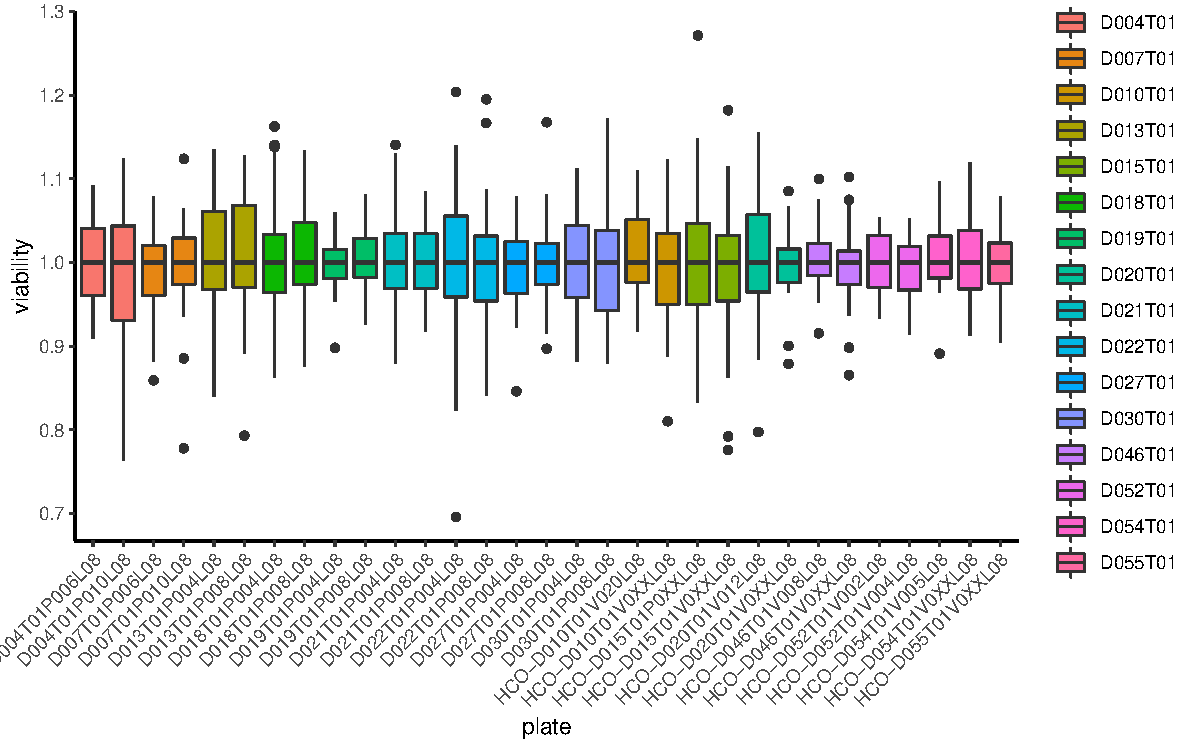
\includegraphics{organoid_unsupervised_exploration_files/figure-latex/unnamed-chunk-10-1.pdf}

\begin{Shaded}
\begin{Highlighting}[]
\NormalTok{organoid_size_factor_}\DecValTok{09}\NormalTok{ <-}\StringTok{ }\NormalTok{umap_df }\OperatorTok\StringTok{ }\KeywordTok{filter}\NormalTok{(partition }\OperatorTok\StringTok{ }\KeywordTok{c}\NormalTok{(}\DecValTok{1}\NormalTok{,}\DecValTok{2}\NormalTok{)) }\OperatorTok\StringTok{ }\KeywordTok{group_by}\NormalTok{(line) }\OperatorTok\StringTok{ }
\StringTok{  }\KeywordTok{summarise}\NormalTok{(}\DataTypeTok{x =} \KeywordTok{quantile}\NormalTok{(size_log, }\FloatTok{0.9}\NormalTok{)) }\OperatorTok\StringTok{ }
\StringTok{  }\CommentTok{#summarise(x = mean(size_log)) %>% }
\StringTok{  }\KeywordTok{arrange}\NormalTok{(x) }\OperatorTok\StringTok{ }\NormalTok{.}\OperatorTok{$}\NormalTok{line}


\NormalTok{gg_size_dist_morph_ridge <-}\StringTok{ }\NormalTok{umap_df_sample }\OperatorTok\StringTok{ }\KeywordTok{filter}\NormalTok{(partition }\OperatorTok\StringTok{ }\KeywordTok{c}\NormalTok{(}\DecValTok{1}\NormalTok{,}\DecValTok{2}\NormalTok{)) }\OperatorTok\StringTok{ }\KeywordTok{filter}\NormalTok{(drug }\OperatorTok{==}\StringTok{ "DMSO"}\NormalTok{) }\OperatorTok\StringTok{ }
\StringTok{  }\KeywordTok{mutate}\NormalTok{(}\DataTypeTok{line =} \KeywordTok{factor}\NormalTok{(line, }\DataTypeTok{levels =}\NormalTok{ organoid_size_factor_}\DecValTok{09}\NormalTok{)) }\OperatorTok\StringTok{ }
\StringTok{  }\KeywordTok{ggplot}\NormalTok{() }\OperatorTok{+}
\StringTok{  }\KeywordTok{geom_density_ridges_gradient}\NormalTok{(}\KeywordTok{aes}\NormalTok{(}\DataTypeTok{y =}\NormalTok{ line, }\DataTypeTok{x =}\NormalTok{ size_log, }\DataTypeTok{fill =} \KeywordTok{stat}\NormalTok{(x)), }\DataTypeTok{scale =} \DecValTok{1}\NormalTok{) }\OperatorTok{+}
\StringTok{  }\CommentTok{#geom_density(aes(x = size_log, group = replicate, color = morphological_class)) + }
\StringTok{  }\CommentTok{#facet_wrap(~ line) + }
\StringTok{  }\KeywordTok{scale_fill_viridis_c}\NormalTok{() }\OperatorTok{+}
\StringTok{  }\KeywordTok{labs}\NormalTok{(}\DataTypeTok{caption =} \StringTok{"DMSO treated organoids"}\NormalTok{,}
       \DataTypeTok{x =} \StringTok{"ln(size)"}\NormalTok{,}
       \DataTypeTok{fill =} \StringTok{"size"}\NormalTok{) }\OperatorTok{+}\StringTok{ }
\StringTok{  }\KeywordTok{theme}\NormalTok{(}\DataTypeTok{legend.position =} \StringTok{"bottom"}\NormalTok{) }\OperatorTok{+}
\StringTok{  }\KeywordTok{theme_cowplot}\NormalTok{() }\OperatorTok{+}\StringTok{ }
\StringTok{  }\KeywordTok{labs}\NormalTok{(}\DataTypeTok{caption =} \StringTok{"DMSO treated, downsampled"}\NormalTok{)}

\NormalTok{gg_size_dist_morph_ridge}
\end{Highlighting}
\end{Shaded}

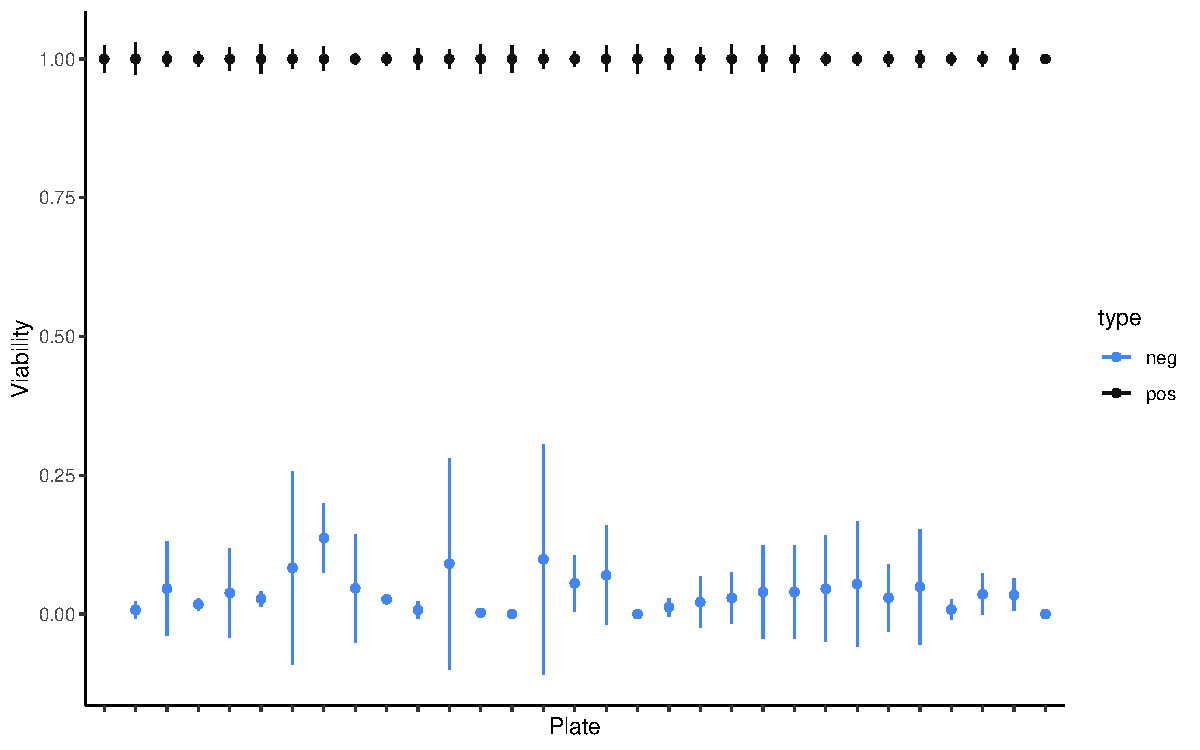
\includegraphics{organoid_unsupervised_exploration_files/figure-latex/unnamed-chunk-11-1.pdf}

\begin{Shaded}
\begin{Highlighting}[]
\NormalTok{umap_size <-}\StringTok{ }\ControlFlowTok{function}\NormalTok{(umap)\{}
\NormalTok{  umap }\OperatorTok
\StringTok{  }\CommentTok{#filter(Size < 1000) %>%}
\StringTok{  }\KeywordTok{ggplot}\NormalTok{(}\KeywordTok{aes}\NormalTok{(v1, v2, }\DataTypeTok{color =}\NormalTok{ size_log)) }\OperatorTok{+}\StringTok{ }
\StringTok{  }\KeywordTok{geom_point_rast}\NormalTok{(}\DataTypeTok{alpha =} \FloatTok{0.5}\NormalTok{, }\DataTypeTok{size =} \FloatTok{0.35}\NormalTok{) }\OperatorTok{+}\StringTok{ }
\StringTok{  }\KeywordTok{scale_color_viridis_c}\NormalTok{() }\OperatorTok{+}
\StringTok{  }\KeywordTok{theme_cowplot}\NormalTok{() }\OperatorTok{+}
\StringTok{  }\KeywordTok{labs}\NormalTok{(}\DataTypeTok{x =} \StringTok{"UMAP 1"}\NormalTok{,}
       \DataTypeTok{y =} \StringTok{"UMAP 2"}\NormalTok{,}
       \DataTypeTok{color =} \StringTok{"ln(size)"}\NormalTok{) }\OperatorTok{+}\StringTok{ }
\StringTok{  }\KeywordTok{theme}\NormalTok{(}\DataTypeTok{legend.position =} \StringTok{"bottom"}\NormalTok{) }\OperatorTok{+}\StringTok{ }
\StringTok{    }\KeywordTok{coord_fixed}\NormalTok{()}
\NormalTok{\}}

\NormalTok{gg_size <-}\StringTok{ }\KeywordTok{umap_size}\NormalTok{(umap_df) }\OperatorTok{+}\StringTok{ }
\StringTok{  }\KeywordTok{labs}\NormalTok{(}\DataTypeTok{caption =} \StringTok{"all treatments, downsampled"}\NormalTok{)}

\NormalTok{gg_size  }\OperatorTok{+}\StringTok{ }\KeywordTok{ggsave}\NormalTok{(}\KeywordTok{paste0}\NormalTok{(PATH, }\StringTok{"reports/figures/imaging/gg_size_all.pdf"}\NormalTok{))}
\end{Highlighting}
\end{Shaded}

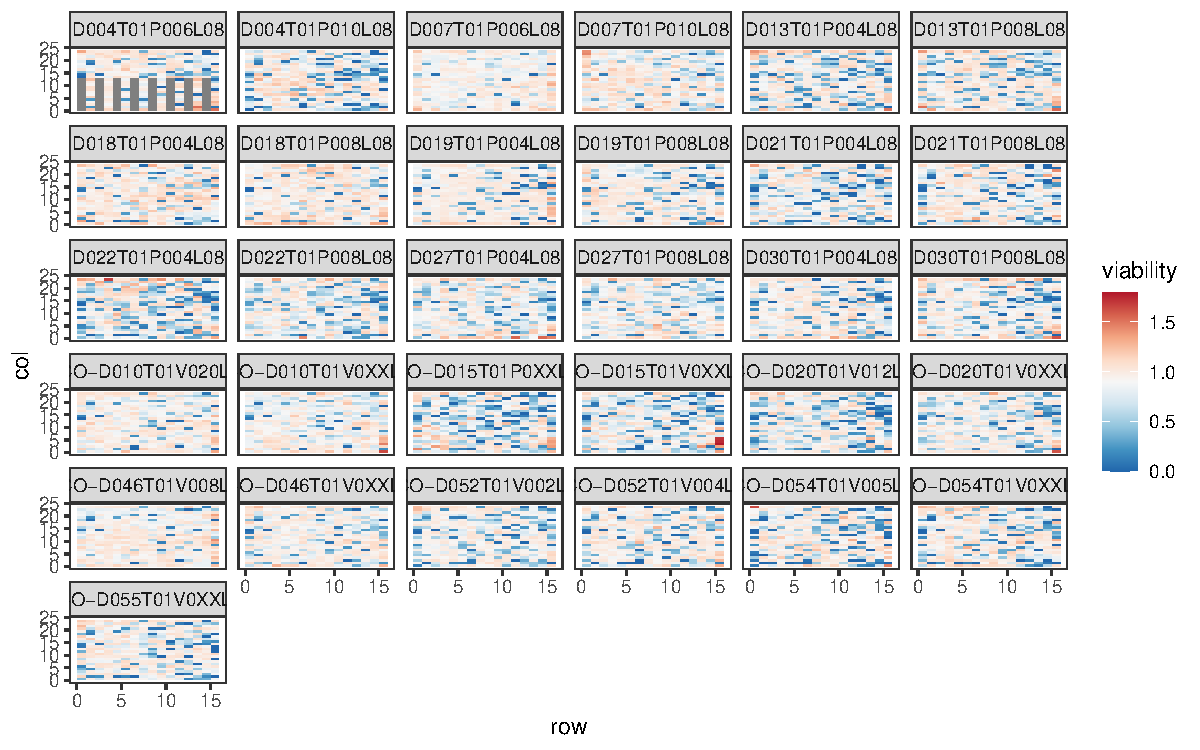
\includegraphics{organoid_unsupervised_exploration_files/figure-latex/unnamed-chunk-12-1.pdf}

In general, DMSO treated organoid lines cover the same latent space than
drug treated organoids. This is likely influenced by the large number of
untreated organoids in the dataset.

\begin{Shaded}
\begin{Highlighting}[]
\NormalTok{df <-}\StringTok{ }\NormalTok{umap_df }

\NormalTok{gg_size_supp <-}\StringTok{ }\NormalTok{df }\OperatorTok
\StringTok{  }\KeywordTok{mutate}\NormalTok{(}\DataTypeTok{drug =} \KeywordTok{if_else}\NormalTok{(drug }\OperatorTok{==}\StringTok{ "DMSO"}\NormalTok{, }\StringTok{"DMSO"}\NormalTok{, }\StringTok{"other"}\NormalTok{)) }\OperatorTok
\StringTok{  }\KeywordTok{ggplot}\NormalTok{(}\KeywordTok{aes}\NormalTok{(v1, v2, }\DataTypeTok{color =}\NormalTok{ size_log)) }\OperatorTok{+}\StringTok{ }
\StringTok{  }\KeywordTok{geom_point_rast}\NormalTok{(}\DataTypeTok{alpha =} \FloatTok{0.5}\NormalTok{, }\DataTypeTok{size =} \FloatTok{0.35}\NormalTok{) }\OperatorTok{+}\StringTok{ }
\StringTok{  }\KeywordTok{scale_color_viridis_c}\NormalTok{() }\OperatorTok{+}
\StringTok{  }\KeywordTok{theme_cowplot}\NormalTok{() }\OperatorTok{+}
\StringTok{  }\KeywordTok{labs}\NormalTok{(}\DataTypeTok{x =} \StringTok{"UMAP 1"}\NormalTok{,}
       \DataTypeTok{y =} \StringTok{"UMAP 2"}\NormalTok{) }\OperatorTok{+}\StringTok{ }
\StringTok{  }\KeywordTok{theme}\NormalTok{(}\DataTypeTok{legend.position =} \StringTok{"bottom"}\NormalTok{) }\OperatorTok{+}
\StringTok{  }\KeywordTok{facet_wrap}\NormalTok{(}\OperatorTok{~}\StringTok{ }\NormalTok{drug) }\OperatorTok{+}\StringTok{ }
\StringTok{  }\KeywordTok{labs}\NormalTok{(}\DataTypeTok{caption =} \StringTok{"downsampled"}\NormalTok{)}

\NormalTok{gg_size_supp }\OperatorTok{+}\StringTok{ }\KeywordTok{ggsave}\NormalTok{(}\KeywordTok{paste0}\NormalTok{(PATH, }\StringTok{"reports/figures/imaging/gg_size_treatment.pdf"}\NormalTok{))}
\end{Highlighting}
\end{Shaded}

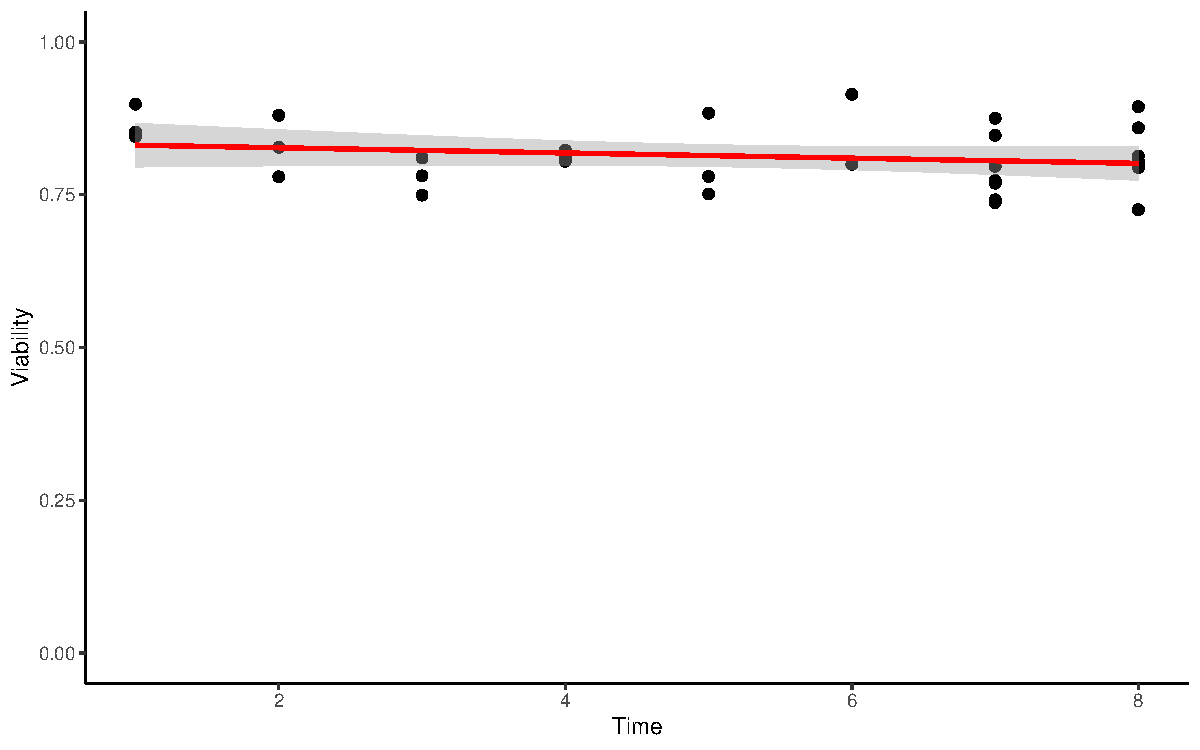
\includegraphics{organoid_unsupervised_exploration_files/figure-latex/unnamed-chunk-13-1.pdf}

\hypertarget{organoid-size-during-drug-treatment}{%
\section{Organoid Size during Drug
Treatment}\label{organoid-size-during-drug-treatment}}

\begin{Shaded}
\begin{Highlighting}[]
\NormalTok{drug_size <-}\StringTok{ }\NormalTok{umap_df_sample }\OperatorTok\StringTok{ }\KeywordTok{filter}\NormalTok{(partition }\OperatorTok\StringTok{ }\KeywordTok{c}\NormalTok{(}\DecValTok{1}\NormalTok{,}\DecValTok{2}\NormalTok{)) }\OperatorTok\StringTok{ }\KeywordTok{filter}\NormalTok{(drug }\OperatorTok{==}\StringTok{ "DMSO"} \OperatorTok{|}\StringTok{ }\NormalTok{drug }\OperatorTok{==}\StringTok{ "Paclitaxel"}\NormalTok{) }\OperatorTok\StringTok{ }
\StringTok{  }\KeywordTok{mutate}\NormalTok{(}\DataTypeTok{concentration =} \KeywordTok{ifelse}\NormalTok{(drug }\OperatorTok{==}\StringTok{ "DMSO"}\NormalTok{, }\DecValTok{0}\NormalTok{, concentration)) }\OperatorTok
\StringTok{  }\CommentTok{#filter(morphological_class == "disorganized") %>% }
\StringTok{  }\CommentTok{#filter(morphological_class != "other") %>% }
\StringTok{  }\KeywordTok{mutate}\NormalTok{(}\DataTypeTok{concentration =} \KeywordTok{factor}\NormalTok{(concentration, }\DataTypeTok{levels =} \KeywordTok{c}\NormalTok{(}\StringTok{"0"}\NormalTok{, }\StringTok{"0.0016"}\NormalTok{, }\StringTok{"0.008"}\NormalTok{, }\StringTok{"0.04"}\NormalTok{, }\StringTok{"0.2"}\NormalTok{, }\StringTok{"1.0"}\NormalTok{)))}

\NormalTok{ggdrug_size <-}\StringTok{ }\KeywordTok{ggplot}\NormalTok{(drug_size) }\OperatorTok{+}
\StringTok{  }\KeywordTok{geom_density}\NormalTok{(}\KeywordTok{aes}\NormalTok{(}\DataTypeTok{x =} \KeywordTok{log}\NormalTok{(size), }\DataTypeTok{group =}\NormalTok{ concentration, }\DataTypeTok{color =}\NormalTok{ concentration), }\DataTypeTok{size =} \FloatTok{1.5}\NormalTok{) }\OperatorTok{+}\StringTok{ }
\StringTok{  }\NormalTok{scico}\OperatorTok{::}\KeywordTok{scale_color_scico_d}\NormalTok{() }\OperatorTok{+}
\StringTok{  }\KeywordTok{theme_cowplot}\NormalTok{() }\OperatorTok{+}\StringTok{ }
\StringTok{  }\CommentTok{#scale_x_continuous(limits = c(0, 15000)) +}
\StringTok{  }\KeywordTok{theme}\NormalTok{(}\DataTypeTok{legend.position =} \StringTok{"bottom"}\NormalTok{) }\OperatorTok{+}\StringTok{ }
\StringTok{  }\KeywordTok{labs}\NormalTok{(}\DataTypeTok{color =} \StringTok{"Paclitaxel Concentration Factor"}\NormalTok{,}
       \DataTypeTok{title =} \StringTok{"Organoid size distribution"}\NormalTok{,}
       \DataTypeTok{x =} \StringTok{"ln(size)"}\NormalTok{)}

\NormalTok{ggdrug_size }
\end{Highlighting}
\end{Shaded}

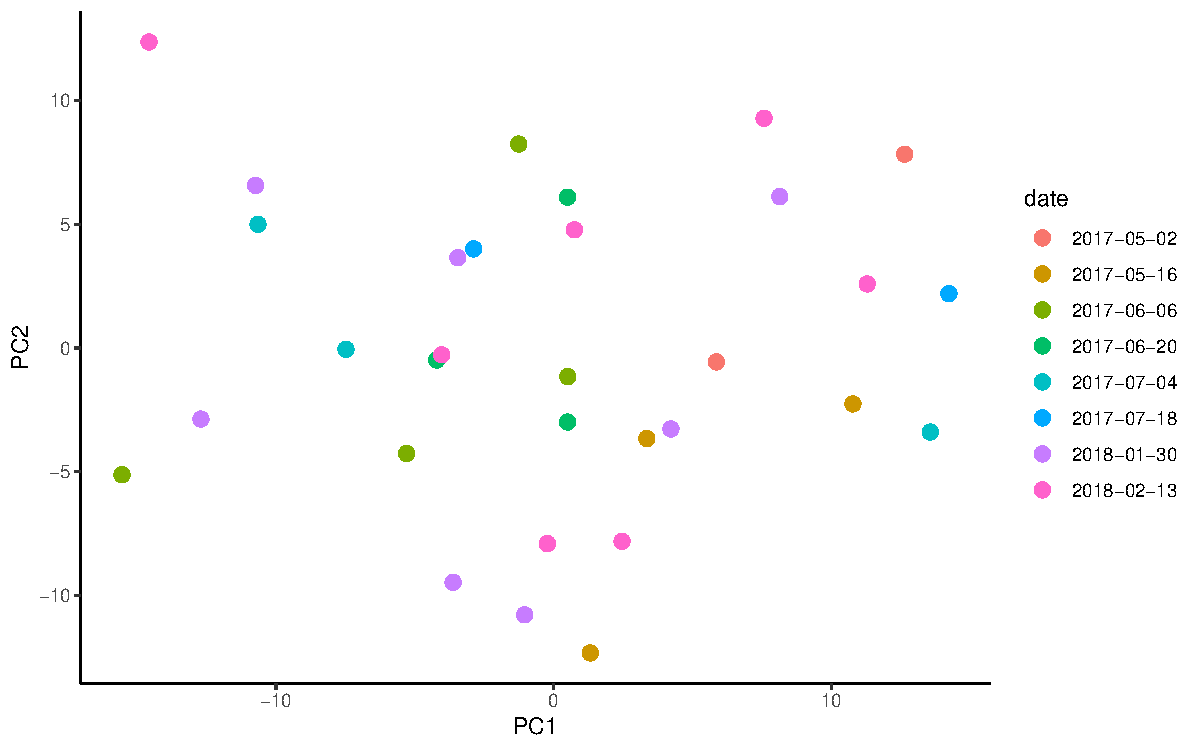
\includegraphics{organoid_unsupervised_exploration_files/figure-latex/unnamed-chunk-14-1.pdf}

\begin{Shaded}
\begin{Highlighting}[]
\NormalTok{drug_count <-}\StringTok{ }\NormalTok{drug_size }\OperatorTok
\StringTok{  }\NormalTok{dplyr}\OperatorTok{::}\KeywordTok{count}\NormalTok{(concentration, line, replicate, well)}

\NormalTok{ggdrug_count <-}\StringTok{ }\KeywordTok{ggplot}\NormalTok{(drug_count) }\OperatorTok{+}
\StringTok{  }\KeywordTok{geom_density}\NormalTok{(}\KeywordTok{aes}\NormalTok{(}\DataTypeTok{x =}\NormalTok{ n, }\DataTypeTok{group =}\NormalTok{ concentration, }\DataTypeTok{color =}\NormalTok{ concentration), }\DataTypeTok{size =} \FloatTok{1.5}\NormalTok{) }\OperatorTok{+}\StringTok{ }
\StringTok{  }\NormalTok{scico}\OperatorTok{::}\KeywordTok{scale_color_scico_d}\NormalTok{() }\OperatorTok{+}
\StringTok{  }\KeywordTok{theme_cowplot}\NormalTok{() }\OperatorTok{+}\StringTok{ }
\StringTok{  }\KeywordTok{theme}\NormalTok{(}\DataTypeTok{legend.position =} \StringTok{"bottom"}\NormalTok{) }\OperatorTok{+}\StringTok{ }
\StringTok{  }\KeywordTok{labs}\NormalTok{(}\DataTypeTok{color =} \StringTok{"Paclitaxel Concentration Factor"}\NormalTok{,}
       \DataTypeTok{title =} \StringTok{"Organoid count distribution"}\NormalTok{,}
       \DataTypeTok{x =} \StringTok{"number of objects per well"}\NormalTok{) }\OperatorTok{+}\StringTok{ }
\StringTok{  }\KeywordTok{scale_x_log10}\NormalTok{()}

\NormalTok{ggdrug_count}
\end{Highlighting}
\end{Shaded}

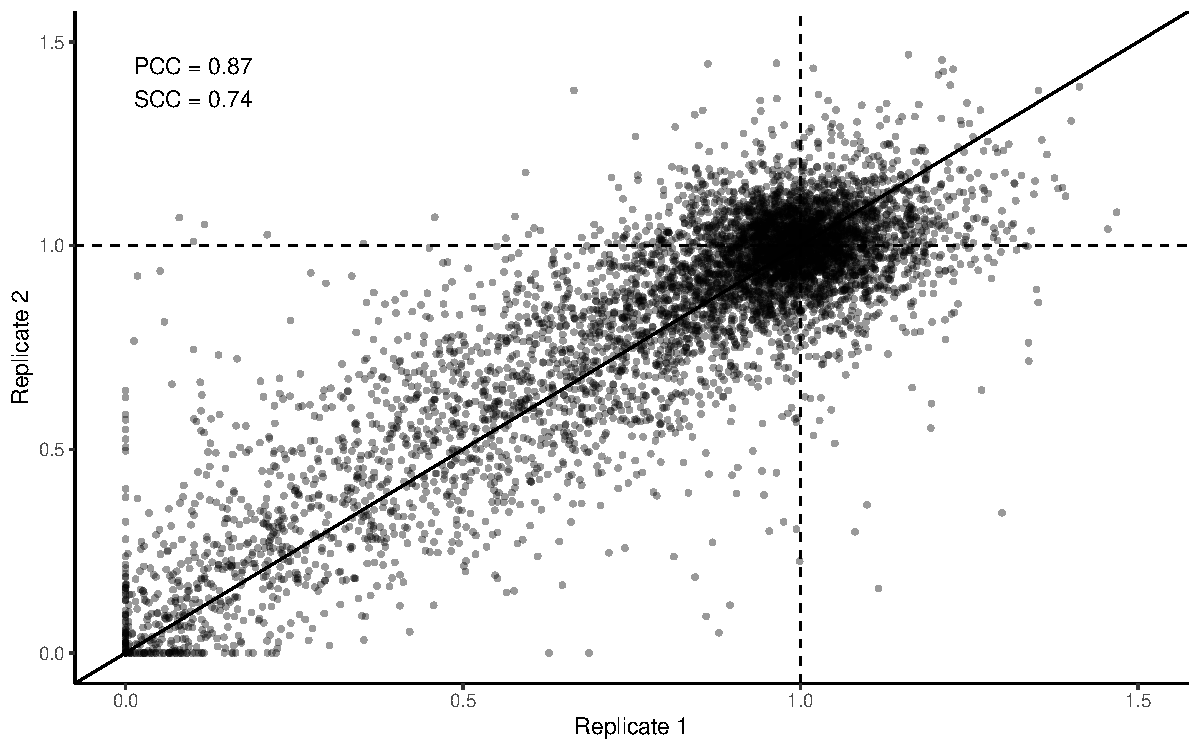
\includegraphics{organoid_unsupervised_exploration_files/figure-latex/unnamed-chunk-15-1.pdf}

\begin{Shaded}
\begin{Highlighting}[]
\KeywordTok{set.seed}\NormalTok{(}\DecValTok{234}\NormalTok{)}
\NormalTok{loi =}\StringTok{ }\KeywordTok{c}\NormalTok{(}\StringTok{"D022T01"}\NormalTok{, }\StringTok{"D046T01"}\NormalTok{)}


\NormalTok{df <-}\StringTok{ }\NormalTok{umap_df_sample  }\OperatorTok
\StringTok{  }\KeywordTok{filter}\NormalTok{(partition }\OperatorTok\StringTok{ }\KeywordTok{c}\NormalTok{(}\DecValTok{1}\NormalTok{,}\DecValTok{2}\NormalTok{)) }\OperatorTok
\StringTok{  }\KeywordTok{filter}\NormalTok{(drug }\OperatorTok{==}\StringTok{ "DMSO"} \OperatorTok{|}\StringTok{ }\NormalTok{drug }\OperatorTok{==}\StringTok{ "Paclitaxel"}\NormalTok{) }\OperatorTok\StringTok{ }
\StringTok{  }\KeywordTok{mutate}\NormalTok{(}\DataTypeTok{concentration =} \KeywordTok{ifelse}\NormalTok{(drug }\OperatorTok{==}\StringTok{ "DMSO"}\NormalTok{, }\DecValTok{0}\NormalTok{, concentration)) }\OperatorTok\StringTok{ }
\StringTok{  }\KeywordTok{filter}\NormalTok{(line }\OperatorTok{==}\StringTok{ }\NormalTok{loi)}

\NormalTok{gg_drug <-}\StringTok{ }\NormalTok{umap_df_sample }\OperatorTok\StringTok{ }\KeywordTok{filter}\NormalTok{(partition }\OperatorTok\StringTok{ }\KeywordTok{c}\NormalTok{(}\DecValTok{1}\NormalTok{,}\DecValTok{2}\NormalTok{)) }\OperatorTok
\StringTok{  }\NormalTok{dplyr}\OperatorTok{::}\KeywordTok{select}\NormalTok{(}\OperatorTok{-}\NormalTok{line, }\OperatorTok{-}\NormalTok{concentration) }\OperatorTok
\StringTok{  }\KeywordTok{ggplot}\NormalTok{(}\KeywordTok{aes}\NormalTok{(v1, v2)) }\OperatorTok{+}\StringTok{ }
\StringTok{  }\KeywordTok{geom_point_rast}\NormalTok{(}\DataTypeTok{alpha =} \DecValTok{1}\NormalTok{, }\DataTypeTok{size =} \FloatTok{0.35}\NormalTok{, }\DataTypeTok{color =} \StringTok{"#f1f1f1"}\NormalTok{) }\OperatorTok{+}\StringTok{ }
\StringTok{  }\KeywordTok{geom_point_rast}\NormalTok{(}\DataTypeTok{data =}\NormalTok{ df  }\OperatorTok
\StringTok{    }\KeywordTok{group_by}\NormalTok{(concentration) }\OperatorTok\StringTok{ }
\StringTok{    }\KeywordTok{sample_n}\NormalTok{(}\DecValTok{1000}\NormalTok{, }\DataTypeTok{replace =} \OtherTok{TRUE}\NormalTok{),}
  \KeywordTok{aes}\NormalTok{(}\DataTypeTok{color =}\NormalTok{ concentration),}\DataTypeTok{alpha =} \DecValTok{1}\NormalTok{, }\DataTypeTok{size =} \FloatTok{1.5}\NormalTok{, }\DataTypeTok{shape=}\DecValTok{16}\NormalTok{) }\OperatorTok{+}\StringTok{ }
\StringTok{  }\CommentTok{#facet_wrap( ~ concentration, ncol = 1) + }
\StringTok{  }\CommentTok{#scale_color_brewer(type = "seq", palette = "YlOrRd") + }
\StringTok{  }\CommentTok{#geom_density2d(color = "black") + }
\StringTok{  }\KeywordTok{theme_classic}\NormalTok{() }\OperatorTok{+}
\StringTok{  }\KeywordTok{labs}\NormalTok{(}\DataTypeTok{x =} \StringTok{"UMAP 1"}\NormalTok{,}
       \DataTypeTok{y =} \StringTok{"UMAP 2"}\NormalTok{,}
       \DataTypeTok{caption =} \KeywordTok{paste0}\NormalTok{(}\KeywordTok{paste}\NormalTok{(loi, }\DataTypeTok{collapse=}\StringTok{" "}\NormalTok{), }\StringTok{", Paclitaxel"}\NormalTok{),}
       \DataTypeTok{color =} \StringTok{"Concentration Factor"}\NormalTok{) }\OperatorTok{+}\StringTok{ }
\StringTok{  }\NormalTok{scico}\OperatorTok{::}\KeywordTok{scale_color_scico_d}\NormalTok{() }\OperatorTok{+}\StringTok{ }
\StringTok{  }\KeywordTok{facet_wrap}\NormalTok{(}\OperatorTok{~}\StringTok{ }\NormalTok{line, }\DataTypeTok{ncol =} \DecValTok{2}\NormalTok{) }\OperatorTok{+}
\StringTok{  }\KeywordTok{theme}\NormalTok{(}\DataTypeTok{legend.position =} \StringTok{"bottom"}\NormalTok{) }\OperatorTok{+}
\StringTok{  }\CommentTok{#theme_cowplot(font_size = 8) + }
\StringTok{  }\KeywordTok{theme}\NormalTok{(}\DataTypeTok{legend.position =} \StringTok{"bottom"}\NormalTok{)}
 
\NormalTok{gg_drug}
\end{Highlighting}
\end{Shaded}

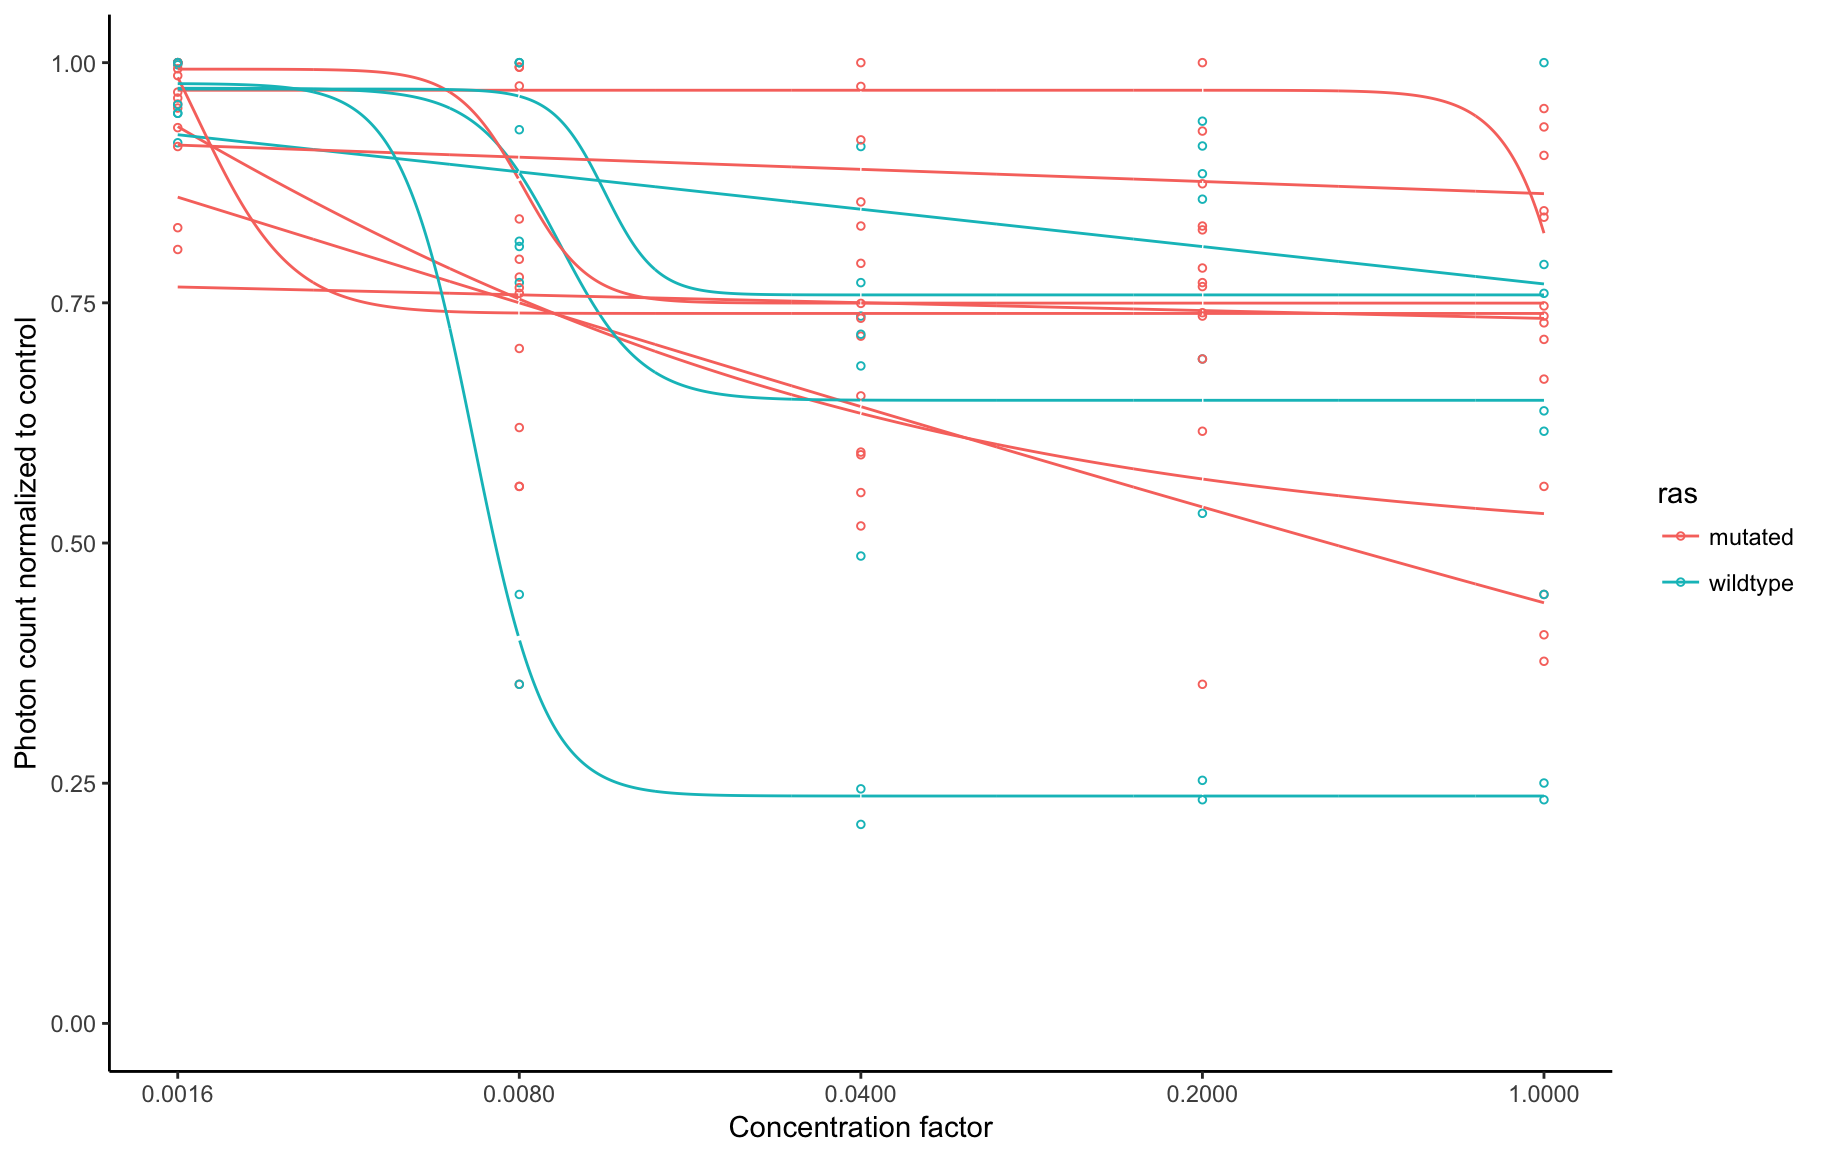
\includegraphics{organoid_unsupervised_exploration_files/figure-latex/unnamed-chunk-16-1.pdf}

\begin{Shaded}
\begin{Highlighting}[]
\NormalTok{loi <-}\StringTok{ }\KeywordTok{c}\NormalTok{(}\StringTok{"D022T01"}\NormalTok{, }\StringTok{"D046T01"}\NormalTok{)}

\NormalTok{drug_size_param <-}\StringTok{ }\NormalTok{drug_size }\OperatorTok\StringTok{ }
\StringTok{  }\KeywordTok{nest}\NormalTok{(}\OperatorTok{-}\NormalTok{concentration, }\OperatorTok{-}\NormalTok{line) }\OperatorTok\StringTok{ }
\StringTok{  }\KeywordTok{mutate}\NormalTok{(}\DataTypeTok{fit =} \KeywordTok{map}\NormalTok{(data, }\OperatorTok{~}\StringTok{ }\NormalTok{fitdistrplus}\OperatorTok{::}\KeywordTok{fitdist}\NormalTok{(.x}\OperatorTok{$}\NormalTok{size, }\StringTok{"lnorm"}\NormalTok{)),}
         \DataTypeTok{param =} \KeywordTok{map}\NormalTok{(fit, }\OperatorTok{~}\StringTok{ }\NormalTok{.x}\OperatorTok{$}\NormalTok{estimate }\OperatorTok\StringTok{ }\NormalTok{broom}\OperatorTok{::}\KeywordTok{tidy}\NormalTok{()))}

\NormalTok{df <-}\StringTok{ }\NormalTok{drug_size_param }\OperatorTok\StringTok{ }\KeywordTok{unnest}\NormalTok{(param) }\OperatorTok\StringTok{ }
\StringTok{  }\KeywordTok{filter}\NormalTok{(names }\OperatorTok{==}\StringTok{ "meanlog"}\NormalTok{) }\OperatorTok
\StringTok{  }\KeywordTok{mutate}\NormalTok{(}\DataTypeTok{concentration =} \KeywordTok{factor}\NormalTok{(concentration, }\DataTypeTok{levels =} \KeywordTok{c}\NormalTok{(}\StringTok{"0"}\NormalTok{, }\StringTok{"0.0016"}\NormalTok{, }\StringTok{"0.008"}\NormalTok{, }\StringTok{"0.04"}\NormalTok{, }\StringTok{"0.2"}\NormalTok{, }\StringTok{"1.0"}\NormalTok{))) }

\NormalTok{gg_size_drug <-}\StringTok{ }\NormalTok{df }\OperatorTok
\StringTok{  }\KeywordTok{filter}\NormalTok{(line }\OperatorTok\StringTok{ }\NormalTok{loi) }\OperatorTok
\StringTok{  }\CommentTok{#mutate(concentration = as.numeric(as.character(concentration))) %>%}
\StringTok{  }\KeywordTok{ggplot}\NormalTok{(}\KeywordTok{aes}\NormalTok{(concentration, x)) }\OperatorTok{+}\StringTok{ }
\StringTok{    }\KeywordTok{geom_point}\NormalTok{(}\DataTypeTok{color =} \StringTok{"grey"}\NormalTok{) }\OperatorTok{+}\StringTok{ }
\StringTok{  }\KeywordTok{geom_line}\NormalTok{(}\DataTypeTok{data =}\NormalTok{ df }\OperatorTok\StringTok{ }\NormalTok{dplyr}\OperatorTok{::}\KeywordTok{rename}\NormalTok{(}\DataTypeTok{line_h =}\NormalTok{ line) , }\KeywordTok{aes}\NormalTok{(}\DataTypeTok{group =}\NormalTok{ line_h), }\DataTypeTok{color =} \StringTok{"grey"}\NormalTok{) }\OperatorTok{+}
\StringTok{  }\KeywordTok{geom_point}\NormalTok{(}\DataTypeTok{data =}\NormalTok{ df }\OperatorTok\StringTok{ }\NormalTok{dplyr}\OperatorTok{::}\KeywordTok{rename}\NormalTok{(}\DataTypeTok{line_h =}\NormalTok{ line), }\DataTypeTok{color =} \StringTok{"grey"}\NormalTok{) }\OperatorTok{+}
\StringTok{  }\KeywordTok{geom_point}\NormalTok{(}\DataTypeTok{color =} \StringTok{"black"}\NormalTok{) }\OperatorTok{+}
\StringTok{  }\KeywordTok{geom_line}\NormalTok{(}\KeywordTok{aes}\NormalTok{(}\DataTypeTok{group =}\NormalTok{ line), }\DataTypeTok{color =} \StringTok{"black"}\NormalTok{) }\OperatorTok{+}
\StringTok{  }\KeywordTok{labs}\NormalTok{(}\DataTypeTok{y =} \StringTok{'mu ln(size)'}\NormalTok{ ,}
       \DataTypeTok{x =} \StringTok{"Concentration Factor"}\NormalTok{,}
       \DataTypeTok{caption =} \KeywordTok{paste0}\NormalTok{(}\KeywordTok{paste}\NormalTok{(loi, }\DataTypeTok{collapse=}\StringTok{" "}\NormalTok{), }\StringTok{", Paclitaxel"}\NormalTok{)) }\OperatorTok{+}
\StringTok{  }\KeywordTok{facet_wrap}\NormalTok{(}\OperatorTok{~}\StringTok{ }\NormalTok{line)}\OperatorTok{+}
\StringTok{  }\KeywordTok{theme_cowplot}\NormalTok{()}

\NormalTok{gg_size_drug}
\end{Highlighting}
\end{Shaded}

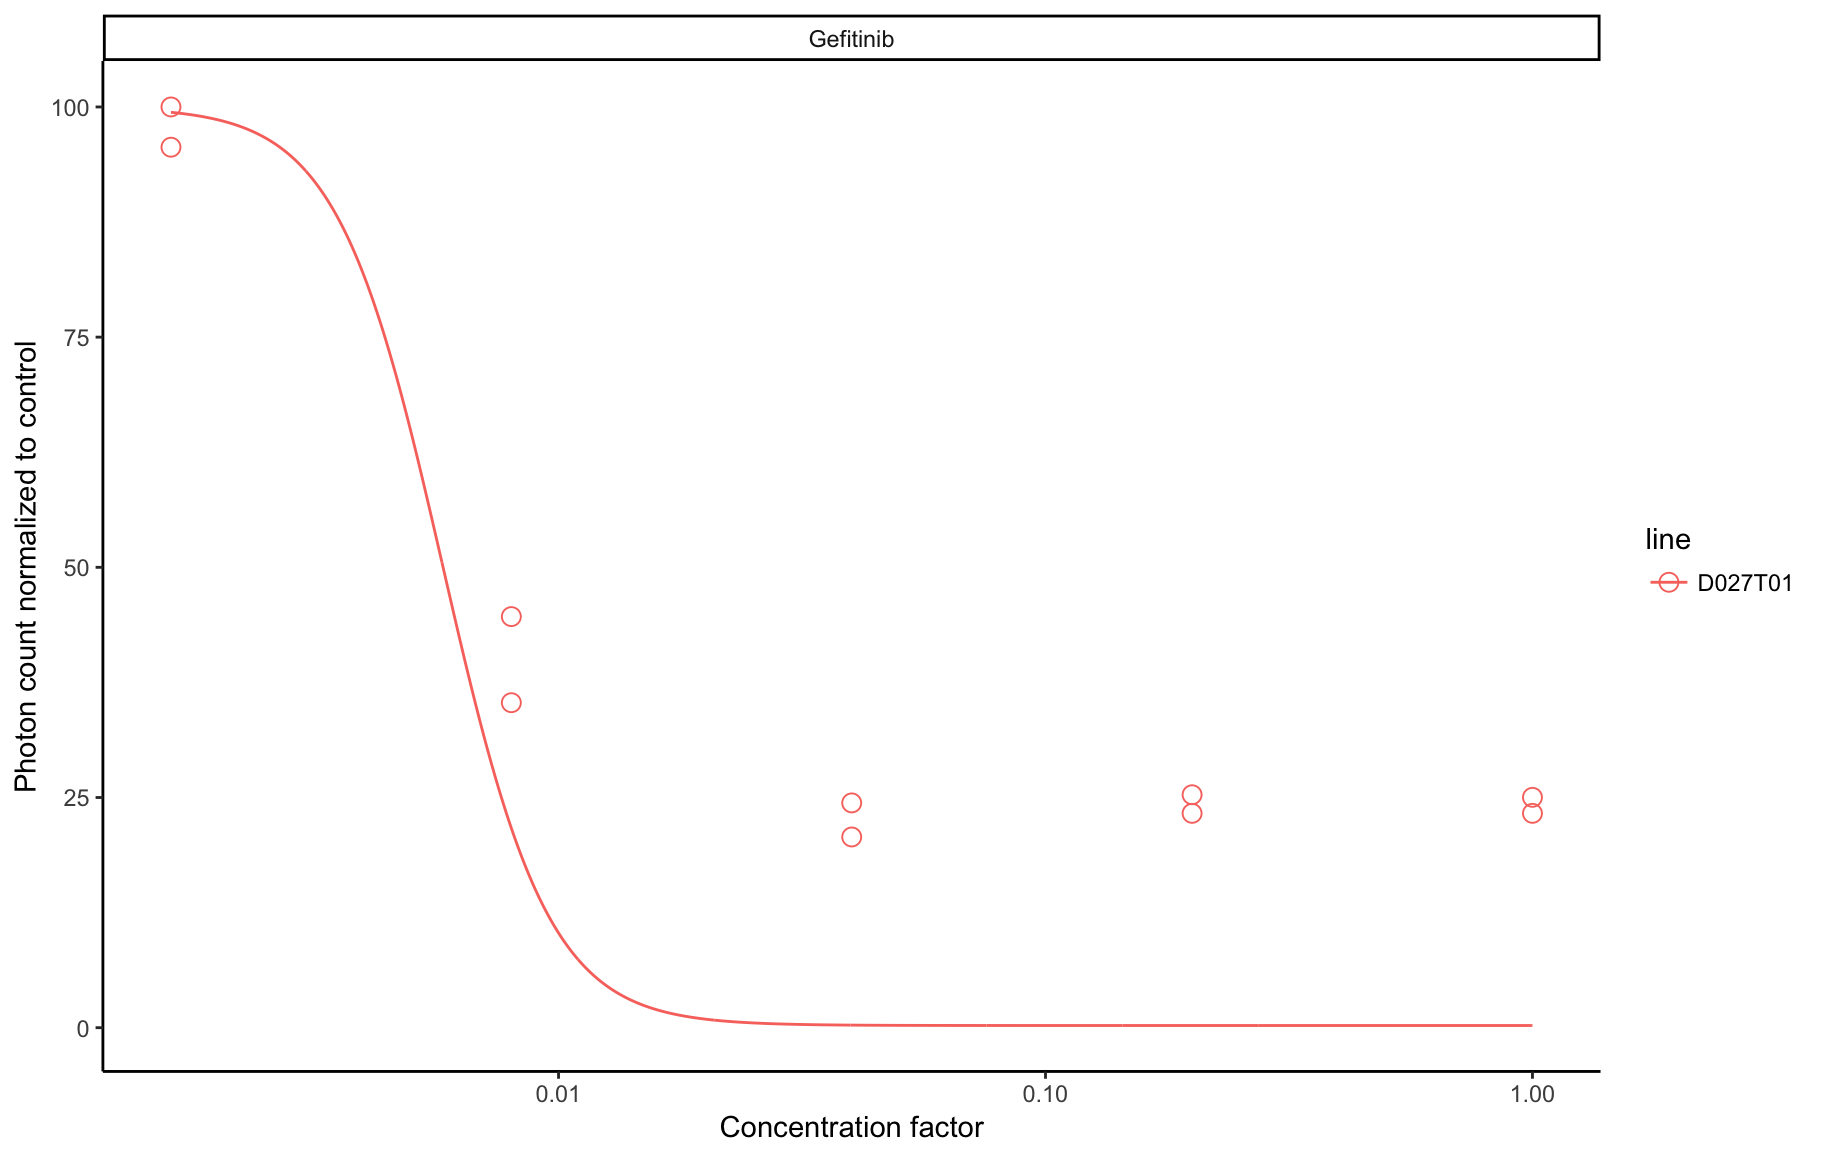
\includegraphics{organoid_unsupervised_exploration_files/figure-latex/unnamed-chunk-17-1.pdf}
\#\# TODO

\begin{Shaded}
\begin{Highlighting}[]
\NormalTok{umap_ldc <-}\StringTok{ }\ControlFlowTok{function}\NormalTok{(umap)\{}
\NormalTok{  umap }\OperatorTok
\StringTok{  }\CommentTok{#filter(Size < 1000) %>%}
\StringTok{  }\KeywordTok{ggplot}\NormalTok{(}\KeywordTok{aes}\NormalTok{(v1, v2, }\DataTypeTok{color =}\NormalTok{ prob_dead)) }\OperatorTok{+}\StringTok{ }
\StringTok{  }\KeywordTok{geom_point_rast}\NormalTok{(}\DataTypeTok{alpha =} \FloatTok{0.5}\NormalTok{, }\DataTypeTok{size =} \FloatTok{0.35}\NormalTok{) }\OperatorTok{+}\StringTok{ }
\StringTok{  }\KeywordTok{scale_color_scico}\NormalTok{(}\DataTypeTok{palette =} \StringTok{'lajolla'}\NormalTok{) }\OperatorTok{+}\StringTok{ }\CommentTok{#lajolla #vikO}
\StringTok{  }\KeywordTok{theme_cowplot}\NormalTok{() }\OperatorTok{+}
\StringTok{  }\KeywordTok{labs}\NormalTok{(}\DataTypeTok{x =} \StringTok{"UMAP 1"}\NormalTok{,}
       \DataTypeTok{y =} \StringTok{"UMAP 2"}\NormalTok{,}
       \DataTypeTok{color =} \StringTok{"p(dead)"}\NormalTok{) }\OperatorTok{+}\StringTok{ }
\StringTok{  }\KeywordTok{theme}\NormalTok{(}\DataTypeTok{legend.position =} \StringTok{"bottom"}\NormalTok{) }\OperatorTok{+}\StringTok{ }
\StringTok{  }\KeywordTok{guides}\NormalTok{(}\DataTypeTok{fill =} \KeywordTok{guide_colourbar}\NormalTok{(}\DataTypeTok{barwidth =} \FloatTok{0.5}\NormalTok{, }\DataTypeTok{barheight =} \DecValTok{10}\NormalTok{))}
\NormalTok{\}}

\NormalTok{gg_ldc <-}\StringTok{ }\KeywordTok{umap_ldc}\NormalTok{(umap_df }\OperatorTok\StringTok{ }\KeywordTok{filter}\NormalTok{(partition }\OperatorTok\StringTok{ }\KeywordTok{c}\NormalTok{(}\DecValTok{1}\NormalTok{,}\DecValTok{2}\NormalTok{)))}

\NormalTok{gg_ldc}
\end{Highlighting}
\end{Shaded}

\hypertarget{organoid-heterogeneity}{%
\section{Organoid Heterogeneity}\label{organoid-heterogeneity}}

I plot 2 organoid lines treated with DMSO control

\begin{Shaded}
\begin{Highlighting}[]
\KeywordTok{set.seed}\NormalTok{(}\DecValTok{234}\NormalTok{)}


\NormalTok{df <-}\StringTok{ }\NormalTok{umap_df  }\OperatorTok\StringTok{ }\KeywordTok{filter}\NormalTok{(partition }\OperatorTok\StringTok{ }\KeywordTok{c}\NormalTok{(}\DecValTok{1}\NormalTok{,}\DecValTok{2}\NormalTok{)) }\OperatorTok
\StringTok{  }\KeywordTok{mutate}\NormalTok{(}\DataTypeTok{cystic =} \KeywordTok{if_else}\NormalTok{(line }\OperatorTok{==}\StringTok{ "D013T01"} \OperatorTok{&}\StringTok{  }\NormalTok{well }\OperatorTok{==}\StringTok{ "D24"} \OperatorTok{&}\StringTok{ }\NormalTok{plate }\OperatorTok{==}\StringTok{ "D013T01P001L02"}\NormalTok{, }\OtherTok{TRUE}\NormalTok{, }\OtherTok{FALSE}\NormalTok{)) }\OperatorTok
\StringTok{  }\KeywordTok{mutate}\NormalTok{(}\DataTypeTok{compact =} \KeywordTok{if_else}\NormalTok{(line }\OperatorTok{==}\StringTok{ "D046T01"} \OperatorTok{&}\StringTok{  }\NormalTok{well }\OperatorTok{==}\StringTok{ "D24"} \OperatorTok{&}\StringTok{ }\NormalTok{plate }\OperatorTok{==}\StringTok{ "D046T01P007L02"}\NormalTok{, }\OtherTok{TRUE}\NormalTok{, }\OtherTok{FALSE}\NormalTok{))}

\NormalTok{gg_cys_comp <-}\StringTok{ }\NormalTok{df }\OperatorTok\StringTok{ }
\StringTok{  }\KeywordTok{sample_frac}\NormalTok{(}\FloatTok{0.01}\NormalTok{) }\OperatorTok
\StringTok{  }\KeywordTok{ggplot}\NormalTok{(}\KeywordTok{aes}\NormalTok{(v1, v2, }\DataTypeTok{color =}\NormalTok{ size_log)) }\OperatorTok{+}\StringTok{ }
\StringTok{  }\CommentTok{#scale_color_brewer(type = "qual", palette = 2) +}
\StringTok{  }\KeywordTok{geom_point_rast}\NormalTok{(}\DataTypeTok{alpha =} \FloatTok{0.1}\NormalTok{, }\DataTypeTok{size =} \FloatTok{0.35}\NormalTok{) }\OperatorTok{+}\StringTok{ }
\StringTok{  }\KeywordTok{geom_point_rast}\NormalTok{(}\DataTypeTok{color =} \StringTok{"#F4B400"}\NormalTok{, }\DataTypeTok{alpha =} \DecValTok{1}\NormalTok{, }\DataTypeTok{size =} \FloatTok{0.5}\NormalTok{, }\DataTypeTok{data =}\NormalTok{ df }\OperatorTok\StringTok{ }\KeywordTok{filter}\NormalTok{(cystic }\OperatorTok{==}\StringTok{ }\OtherTok{TRUE}\NormalTok{)) }\OperatorTok{+}
\StringTok{  }\KeywordTok{geom_point_rast}\NormalTok{(}\DataTypeTok{color =} \StringTok{"#DB4437"}\NormalTok{, }\DataTypeTok{alpha =} \DecValTok{1}\NormalTok{, }\DataTypeTok{size =} \FloatTok{0.5}\NormalTok{, }\DataTypeTok{data =}\NormalTok{ df }\OperatorTok\StringTok{ }\KeywordTok{filter}\NormalTok{(compact }\OperatorTok{==}\StringTok{ }\OtherTok{TRUE}\NormalTok{)) }\OperatorTok{+}\StringTok{ }
\StringTok{  }\KeywordTok{scale_color_viridis_c}\NormalTok{() }\OperatorTok{+}
\StringTok{  }\KeywordTok{labs}\NormalTok{(}\DataTypeTok{color =} \StringTok{"size"}\NormalTok{,}
       \DataTypeTok{caption =} \StringTok{"yellow: D013T01, red: D055T01"}\NormalTok{,}
       \DataTypeTok{x =} \StringTok{"UMAP 1"}\NormalTok{,}
       \DataTypeTok{y =} \StringTok{"UMAP 2"}\NormalTok{) }\OperatorTok{+}
\StringTok{  }\KeywordTok{theme_cowplot}\NormalTok{() }\OperatorTok{+}\StringTok{ }
\StringTok{  }\KeywordTok{coord_fixed}\NormalTok{()}

\NormalTok{gg_cys_comp}
\end{Highlighting}
\end{Shaded}

\hypertarget{organoid-line-differences}{%
\section{Organoid line differences}\label{organoid-line-differences}}

I create a single plot showing the two extreme organoid lines and their
distribution within the embedding.

\begin{Shaded}
\begin{Highlighting}[]
\KeywordTok{set.seed}\NormalTok{(}\DecValTok{123}\NormalTok{)}

\NormalTok{loi <-}\StringTok{ }\KeywordTok{c}\NormalTok{(}\StringTok{"D019T01"}\NormalTok{, }\StringTok{"D007T01"}\NormalTok{,  }\StringTok{"D030T01"}\NormalTok{, }\StringTok{"D018T01"}\NormalTok{) }\CommentTok{#c("D055T01", "D007T01",  "D021T01", "D019T01", "D027T01")}
\CommentTok{#loi <- umap_df$line %>% unique()}

\NormalTok{df <-}\StringTok{ }\NormalTok{umap_df }\OperatorTok
\StringTok{  }\KeywordTok{filter}\NormalTok{(drug }\OperatorTok{==}\StringTok{ "DMSO"}\NormalTok{) }\OperatorTok\StringTok{ }
\StringTok{  }\KeywordTok{filter}\NormalTok{(partition }\OperatorTok\StringTok{ }\KeywordTok{c}\NormalTok{(}\DecValTok{1}\NormalTok{,}\DecValTok{2}\NormalTok{))}


\NormalTok{gg_line <-}\StringTok{ }\NormalTok{df }\OperatorTok\StringTok{ }\NormalTok{dplyr}\OperatorTok{::}\KeywordTok{select}\NormalTok{(}\OperatorTok{-}\NormalTok{line) }\OperatorTok
\StringTok{  }\KeywordTok{ggplot}\NormalTok{(}\KeywordTok{aes}\NormalTok{(v1, v2)) }\OperatorTok{+}\StringTok{ }
\StringTok{  }\KeywordTok{geom_point_rast}\NormalTok{(}\DataTypeTok{alpha =} \DecValTok{1}\NormalTok{, }\DataTypeTok{size =} \FloatTok{0.35}\NormalTok{, }\DataTypeTok{color =} \StringTok{"#f1f1f1"}\NormalTok{) }\OperatorTok{+}\StringTok{ }
\StringTok{  }\KeywordTok{geom_point_rast}\NormalTok{(}\DataTypeTok{data =}\NormalTok{ umap_df }\OperatorTok
\StringTok{                    }\KeywordTok{filter}\NormalTok{(drug }\OperatorTok{==}\StringTok{ "DMSO"}\NormalTok{) }\OperatorTok\StringTok{ }
\StringTok{                   }\CommentTok{# filter(line %in% c("D021T01")) %>%}
\StringTok{    }\KeywordTok{filter}\NormalTok{(line }\OperatorTok\StringTok{ }\NormalTok{loi) }\OperatorTok\StringTok{ }
\StringTok{    }\KeywordTok{mutate}\NormalTok{(}\DataTypeTok{line =} \KeywordTok{factor}\NormalTok{(line, }\DataTypeTok{levels =}\NormalTok{ loi)), }\CommentTok{#%>% }
      \CommentTok{#sample_frac(0.1),}
    \CommentTok{#mutate(line = factor(line, levels = c("D021T01"))),}
  \KeywordTok{aes}\NormalTok{(}\DataTypeTok{color =}\NormalTok{ line),}\DataTypeTok{alpha =} \FloatTok{.4}\NormalTok{, }\DataTypeTok{size =} \FloatTok{0.35}\NormalTok{, }\DataTypeTok{shape=}\DecValTok{16}\NormalTok{) }\OperatorTok{+}\StringTok{ }
\StringTok{  }\KeywordTok{facet_wrap}\NormalTok{( }\OperatorTok{~}\StringTok{ }\NormalTok{line, }\DataTypeTok{ncol =}\DecValTok{2}\NormalTok{) }\OperatorTok{+}
\StringTok{  }\KeywordTok{scale_color_brewer}\NormalTok{(}\DataTypeTok{type =} \StringTok{"qual"}\NormalTok{, }\DataTypeTok{palette =} \StringTok{"Set2"}\NormalTok{) }\OperatorTok{+}
\StringTok{  }\CommentTok{#scale_color_manual(values = c(c("#D80D12", "#461C01", "#9a4c91", "#70BE6F", "#24345E"))) +   }
\StringTok{  }\CommentTok{#geom_density2d(color = "black") + }
\StringTok{  }\KeywordTok{theme_classic}\NormalTok{() }\OperatorTok{+}
\StringTok{  }\KeywordTok{labs}\NormalTok{(}\DataTypeTok{x =} \StringTok{"UMAP 1"}\NormalTok{,}
       \DataTypeTok{y =} \StringTok{"UMAP 2"}\NormalTok{)}\OperatorTok{+}
\StringTok{       }\CommentTok{#caption = "control treated organoids") + }
\StringTok{  }\KeywordTok{theme_cowplot}\NormalTok{(}\DataTypeTok{font_size =} \DecValTok{8}\NormalTok{) }\OperatorTok{+}\StringTok{ }
\StringTok{  }\KeywordTok{theme}\NormalTok{(}\DataTypeTok{legend.position =} \StringTok{"nothing"}\NormalTok{)}

\NormalTok{gg_line }\OperatorTok{+}\StringTok{ }\KeywordTok{ggsave}\NormalTok{(}\KeywordTok{paste0}\NormalTok{(PATH, }\StringTok{"reports/figures/imaging/gg_size_four_lines.pdf"}\NormalTok{), }\DataTypeTok{width =} \DecValTok{4}\NormalTok{, }\DataTypeTok{height =} \DecValTok{4}\NormalTok{)}
\end{Highlighting}
\end{Shaded}

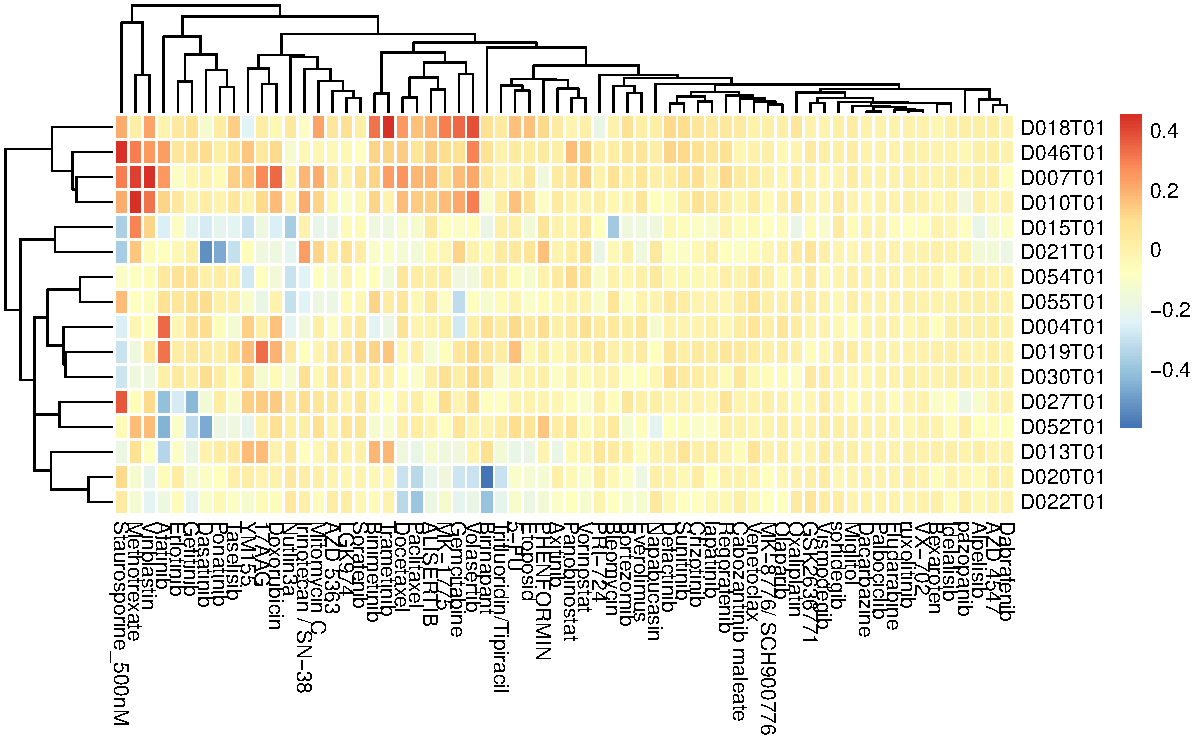
\includegraphics{organoid_unsupervised_exploration_files/figure-latex/unnamed-chunk-20-1.pdf}

\begin{Shaded}
\begin{Highlighting}[]
\NormalTok{df <-}\StringTok{ }\NormalTok{umap_df }\OperatorTok
\StringTok{  }\KeywordTok{left_join}\NormalTok{(organoid_morphology }\OperatorTok\StringTok{ }\KeywordTok{mutate}\NormalTok{(}\DataTypeTok{line =} \KeywordTok{paste0}\NormalTok{(line, }\StringTok{"01"}\NormalTok{))) }\OperatorTok
\StringTok{  }\KeywordTok{filter}\NormalTok{(drug }\OperatorTok{==}\StringTok{ "DMSO"}\NormalTok{) }\OperatorTok\StringTok{ }
\StringTok{  }\KeywordTok{filter}\NormalTok{(partition }\OperatorTok\StringTok{ }\KeywordTok{c}\NormalTok{(}\DecValTok{1}\NormalTok{,}\DecValTok{2}\NormalTok{))}

\NormalTok{gg_morph <-}\StringTok{ }\NormalTok{df }\OperatorTok\StringTok{ }\NormalTok{dplyr}\OperatorTok{::}\KeywordTok{select}\NormalTok{(}\OperatorTok{-}\NormalTok{line) }\OperatorTok
\StringTok{  }\KeywordTok{ggplot}\NormalTok{(}\KeywordTok{aes}\NormalTok{(v1, v2)) }\OperatorTok{+}\StringTok{ }
\StringTok{  }\KeywordTok{geom_point_rast}\NormalTok{(}\DataTypeTok{alpha =} \DecValTok{1}\NormalTok{, }\DataTypeTok{size =} \FloatTok{0.35}\NormalTok{, }\DataTypeTok{color =} \StringTok{"#f1f1f1"}\NormalTok{) }\OperatorTok{+}\StringTok{ }
\StringTok{  }\KeywordTok{geom_point_rast}\NormalTok{(}\DataTypeTok{data =}\NormalTok{ umap_df }\OperatorTok\StringTok{ }\KeywordTok{left_join}\NormalTok{(organoid_morphology }\OperatorTok\StringTok{ }\KeywordTok{mutate}\NormalTok{(}\DataTypeTok{line =} \KeywordTok{paste0}\NormalTok{(line, }\StringTok{"01"}\NormalTok{))) }\OperatorTok
\StringTok{                    }\KeywordTok{filter}\NormalTok{(drug }\OperatorTok{==}\StringTok{ "DMSO"}\NormalTok{), }\CommentTok{#%>% }
      \CommentTok{#sample_frac(0.1),}
    \CommentTok{#mutate(line = factor(line, levels = c("D021T01"))),}
  \KeywordTok{aes}\NormalTok{(}\DataTypeTok{color =}\NormalTok{ morphology),}\DataTypeTok{alpha =} \FloatTok{.4}\NormalTok{, }\DataTypeTok{size =} \FloatTok{0.35}\NormalTok{, }\DataTypeTok{shape=}\DecValTok{16}\NormalTok{) }\OperatorTok{+}\StringTok{ }
\StringTok{  }\CommentTok{#facet_wrap( ~ line, ncol =2) +}
\StringTok{  }\KeywordTok{scale_color_brewer}\NormalTok{(}\DataTypeTok{type =} \StringTok{"qual"}\NormalTok{, }\DataTypeTok{palette =} \StringTok{"Set1"}\NormalTok{) }\OperatorTok{+}
\StringTok{  }\CommentTok{#scale_color_manual(values = c(c("#D80D12", "#461C01", "#9a4c91", "#70BE6F", "#24345E"))) +   }
\StringTok{  }\CommentTok{#geom_density2d(color = "black") + }
\StringTok{  }\KeywordTok{theme_classic}\NormalTok{() }\OperatorTok{+}
\StringTok{  }\KeywordTok{labs}\NormalTok{(}\DataTypeTok{x =} \StringTok{"UMAP 1"}\NormalTok{,}
       \DataTypeTok{y =} \StringTok{"UMAP 2"}\NormalTok{)}\OperatorTok{+}
\StringTok{       }\CommentTok{#caption = "control treated organoids") + }
\StringTok{  }\KeywordTok{theme_cowplot}\NormalTok{(}\DataTypeTok{font_size =} \DecValTok{8}\NormalTok{)}

\NormalTok{gg_morph }\OperatorTok{+}\StringTok{ }\KeywordTok{ggsave}\NormalTok{(}\KeywordTok{paste0}\NormalTok{(PATH, }\StringTok{"reports/figures/imaging/gg_morphology.pdf"}\NormalTok{), }\DataTypeTok{width =} \DecValTok{4}\NormalTok{, }\DataTypeTok{height =} \DecValTok{4}\NormalTok{)}
\end{Highlighting}
\end{Shaded}

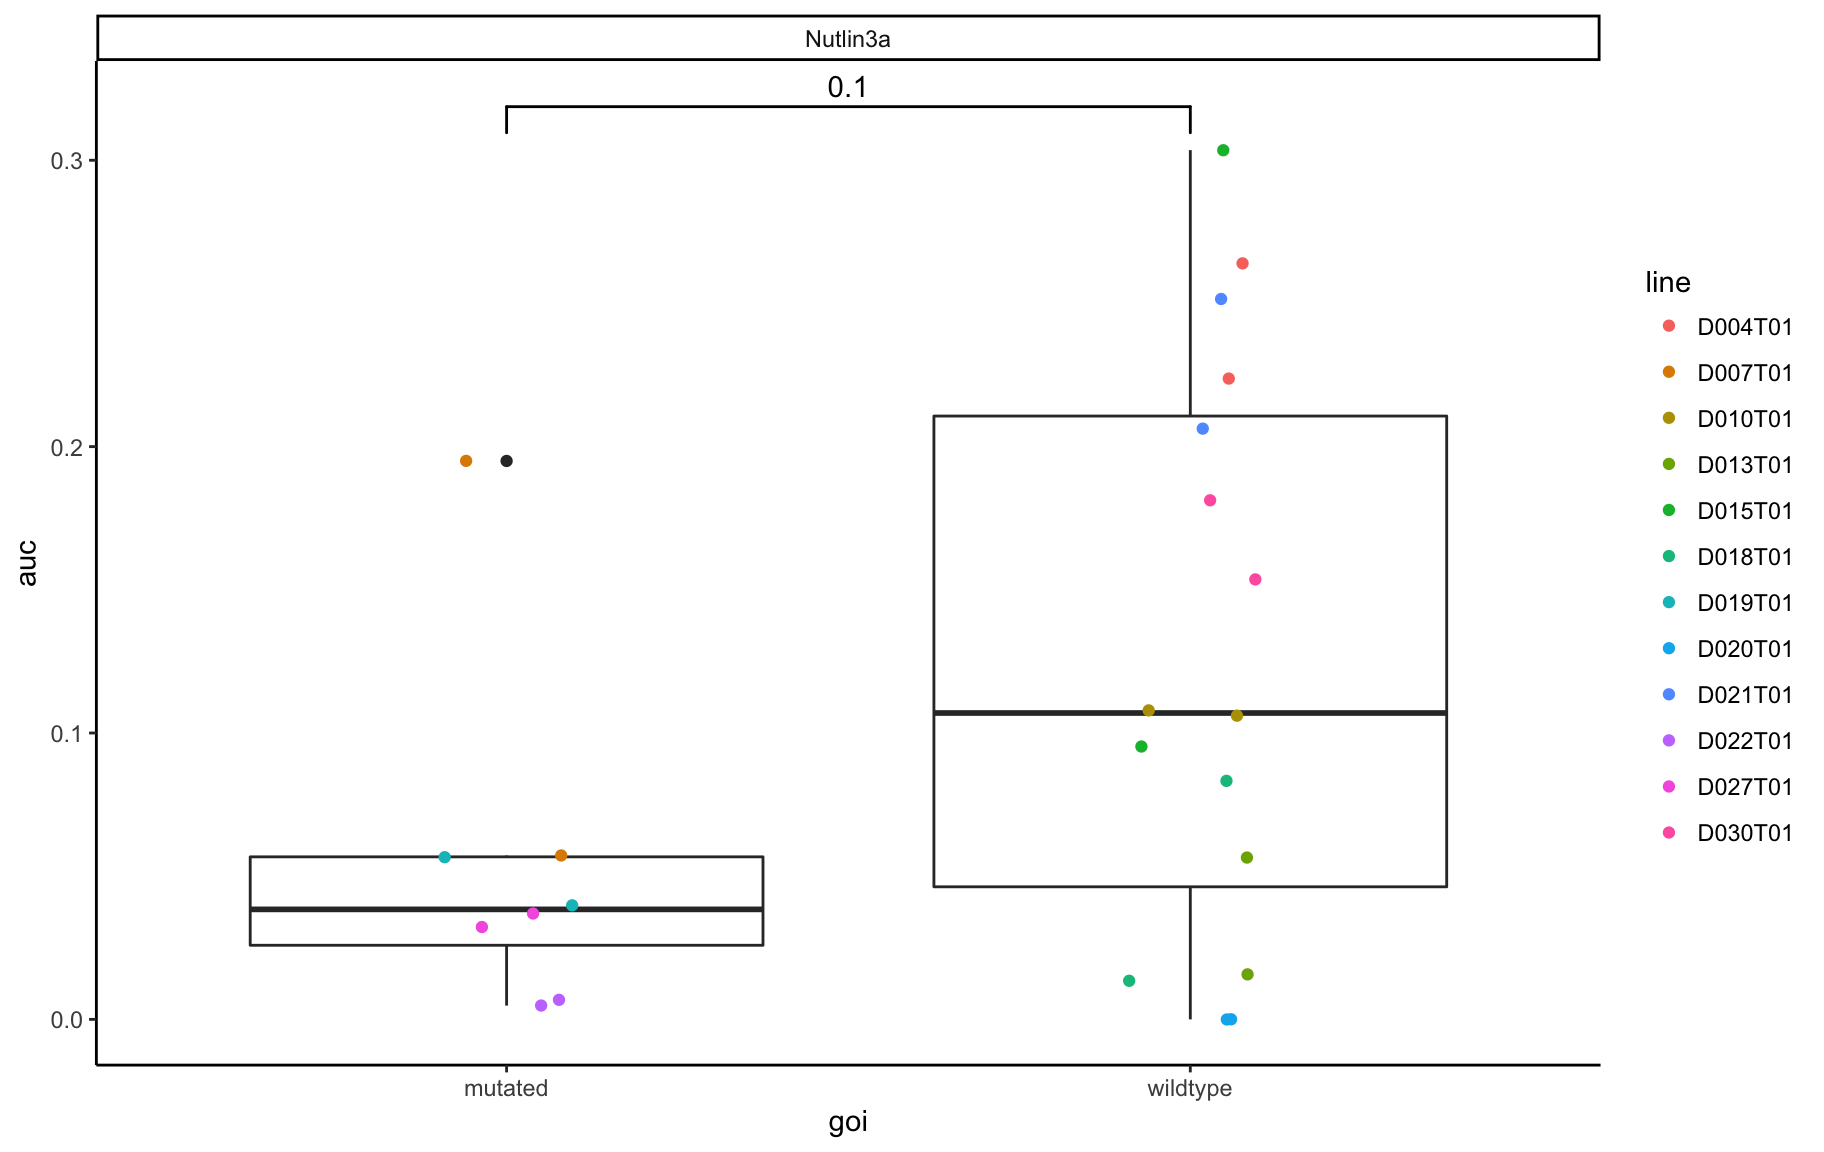
\includegraphics{organoid_unsupervised_exploration_files/figure-latex/unnamed-chunk-21-1.pdf}

\begin{Shaded}
\begin{Highlighting}[]
\NormalTok{df <-}\StringTok{ }\NormalTok{umap_df }\OperatorTok
\StringTok{  }\KeywordTok{left_join}\NormalTok{(organoid_morphology }\OperatorTok\StringTok{ }\KeywordTok{mutate}\NormalTok{(}\DataTypeTok{line =} \KeywordTok{paste0}\NormalTok{(line, }\StringTok{"01"}\NormalTok{))) }\OperatorTok
\StringTok{  }\KeywordTok{filter}\NormalTok{(drug }\OperatorTok{==}\StringTok{ "DMSO"}\NormalTok{) }\OperatorTok\StringTok{ }
\StringTok{  }\KeywordTok{filter}\NormalTok{(partition }\OperatorTok\StringTok{ }\KeywordTok{c}\NormalTok{(}\DecValTok{1}\NormalTok{,}\DecValTok{2}\NormalTok{))}

\NormalTok{gg_screen_id <-}\StringTok{ }\NormalTok{df }\OperatorTok\StringTok{ }\NormalTok{dplyr}\OperatorTok{::}\KeywordTok{select}\NormalTok{(}\OperatorTok{-}\NormalTok{line) }\OperatorTok
\StringTok{  }\KeywordTok{ggplot}\NormalTok{(}\KeywordTok{aes}\NormalTok{(v1, v2)) }\OperatorTok{+}\StringTok{ }
\StringTok{  }\KeywordTok{geom_point_rast}\NormalTok{(}\DataTypeTok{alpha =} \DecValTok{1}\NormalTok{, }\DataTypeTok{size =} \FloatTok{0.35}\NormalTok{, }\DataTypeTok{color =} \StringTok{"#f1f1f1"}\NormalTok{) }\OperatorTok{+}\StringTok{ }
\StringTok{  }\KeywordTok{geom_point_rast}\NormalTok{(}\DataTypeTok{data =}\NormalTok{ umap_df }\OperatorTok\StringTok{ }\KeywordTok{left_join}\NormalTok{(organoid_morphology }\OperatorTok\StringTok{ }\KeywordTok{mutate}\NormalTok{(}\DataTypeTok{line =} \KeywordTok{paste0}\NormalTok{(line, }\StringTok{"01"}\NormalTok{))) }\OperatorTok
\StringTok{                    }\KeywordTok{filter}\NormalTok{(drug }\OperatorTok{==}\StringTok{ "DMSO"}\NormalTok{), }\CommentTok{#%>% }
      \CommentTok{#sample_frac(0.1),}
    \CommentTok{#mutate(line = factor(line, levels = c("D021T01"))),}
  \KeywordTok{aes}\NormalTok{(}\DataTypeTok{color =}\NormalTok{ screen_id),}\DataTypeTok{alpha =} \FloatTok{.4}\NormalTok{, }\DataTypeTok{size =} \FloatTok{0.35}\NormalTok{, }\DataTypeTok{shape=}\DecValTok{16}\NormalTok{) }\OperatorTok{+}\StringTok{ }
\StringTok{  }\KeywordTok{facet_wrap}\NormalTok{( }\OperatorTok{~}\StringTok{ }\NormalTok{line, }\DataTypeTok{ncol =}\DecValTok{4}\NormalTok{) }\OperatorTok{+}
\StringTok{  }\KeywordTok{scale_color_brewer}\NormalTok{(}\DataTypeTok{type =} \StringTok{"qual"}\NormalTok{, }\DataTypeTok{palette =} \StringTok{"Set2"}\NormalTok{) }\OperatorTok{+}
\StringTok{  }\CommentTok{#scale_color_manual(values = c(c("#D80D12", "#461C01", "#9a4c91", "#70BE6F", "#24345E"))) +   }
\StringTok{  }\CommentTok{#geom_density2d(color = "black") + }
\StringTok{  }\KeywordTok{theme_classic}\NormalTok{() }\OperatorTok{+}
\StringTok{  }\KeywordTok{labs}\NormalTok{(}\DataTypeTok{x =} \StringTok{"UMAP 1"}\NormalTok{,}
       \DataTypeTok{y =} \StringTok{"UMAP 2"}\NormalTok{)}\OperatorTok{+}
\StringTok{       }\CommentTok{#caption = "control treated organoids") + }
\StringTok{  }\KeywordTok{theme_cowplot}\NormalTok{(}\DataTypeTok{font_size =} \DecValTok{8}\NormalTok{) }\OperatorTok{+}\StringTok{ }
\StringTok{  }\KeywordTok{theme}\NormalTok{(}\DataTypeTok{legend.position =} \StringTok{"bottom"}\NormalTok{)}

\NormalTok{gg_screen_id }\OperatorTok{+}\StringTok{ }\KeywordTok{ggsave}\NormalTok{(}\KeywordTok{paste0}\NormalTok{(PATH, }\StringTok{"reports/figures/imaging/gg_screen_id.pdf"}\NormalTok{), }\DataTypeTok{width =} \DecValTok{4}\NormalTok{, }\DataTypeTok{height =} \DecValTok{4}\NormalTok{)}
\end{Highlighting}
\end{Shaded}

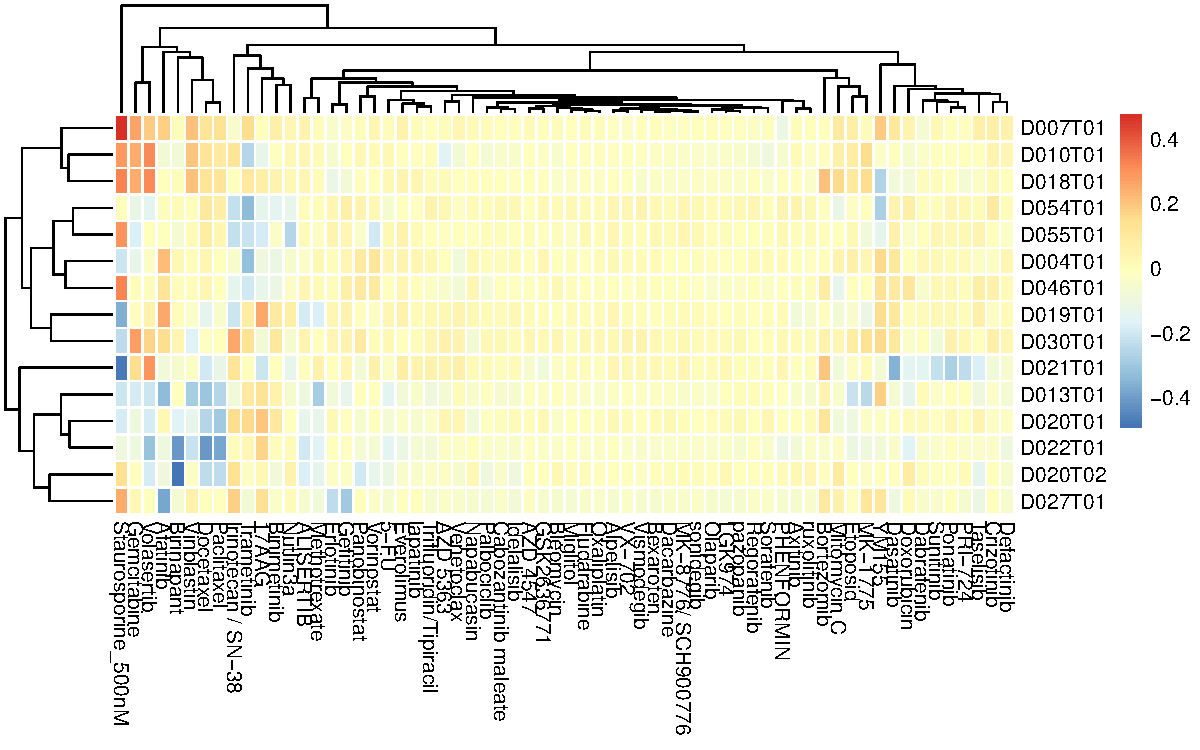
\includegraphics{organoid_unsupervised_exploration_files/figure-latex/unnamed-chunk-22-1.pdf}

\hypertarget{dye-intensity}{%
\section{Dye Intensity}\label{dye-intensity}}

\begin{Shaded}
\begin{Highlighting}[]
\NormalTok{umap_sample }\OperatorTok
\StringTok{  }\KeywordTok{ggplot}\NormalTok{(}\KeywordTok{aes}\NormalTok{(actin, }\DataTypeTok{fill =}\NormalTok{ screen_id)) }\OperatorTok{+}
\StringTok{  }\KeywordTok{geom_density}\NormalTok{(}\DataTypeTok{alpha =} \FloatTok{0.5}\NormalTok{) }\OperatorTok{+}\StringTok{ }
\StringTok{  }\KeywordTok{scale_fill_brewer}\NormalTok{(}\DataTypeTok{type =} \StringTok{'qual'}\NormalTok{) }\OperatorTok{+}
\StringTok{  }\KeywordTok{facet_wrap}\NormalTok{(}\OperatorTok{~}\StringTok{ }\NormalTok{line) }\OperatorTok{+}
\StringTok{  }\KeywordTok{theme_cowplot}\NormalTok{()}
\end{Highlighting}
\end{Shaded}

\begin{Shaded}
\begin{Highlighting}[]
\NormalTok{df }\OperatorTok
\StringTok{  }\KeywordTok{ggplot}\NormalTok{(}\KeywordTok{aes}\NormalTok{(permeability, }\DataTypeTok{fill =}\NormalTok{ screen_id)) }\OperatorTok{+}
\StringTok{  }\KeywordTok{geom_density}\NormalTok{(}\DataTypeTok{alpha =} \FloatTok{0.5}\NormalTok{) }\OperatorTok{+}\StringTok{ }
\StringTok{  }\KeywordTok{scale_fill_brewer}\NormalTok{(}\DataTypeTok{type =} \StringTok{'qual'}\NormalTok{) }\OperatorTok{+}
\StringTok{  }\KeywordTok{facet_wrap}\NormalTok{(}\OperatorTok{~}\StringTok{ }\NormalTok{line) }\OperatorTok{+}
\StringTok{  }\KeywordTok{theme_cowplot}\NormalTok{()}
\end{Highlighting}
\end{Shaded}

\begin{Shaded}
\begin{Highlighting}[]
\NormalTok{df }\OperatorTok
\StringTok{  }\KeywordTok{ggplot}\NormalTok{(}\KeywordTok{aes}\NormalTok{(dapi, }\DataTypeTok{fill =}\NormalTok{ screen_id)) }\OperatorTok{+}
\StringTok{  }\KeywordTok{geom_density}\NormalTok{(}\DataTypeTok{alpha =} \FloatTok{0.5}\NormalTok{) }\OperatorTok{+}\StringTok{ }
\StringTok{  }\KeywordTok{scale_fill_brewer}\NormalTok{(}\DataTypeTok{type =} \StringTok{'qual'}\NormalTok{) }\OperatorTok{+}
\StringTok{  }\KeywordTok{facet_wrap}\NormalTok{(}\OperatorTok{~}\StringTok{ }\NormalTok{line) }\OperatorTok{+}
\StringTok{  }\KeywordTok{theme_cowplot}\NormalTok{()}
\end{Highlighting}
\end{Shaded}

\begin{Shaded}
\begin{Highlighting}[]
\KeywordTok{set.seed}\NormalTok{(}\DecValTok{123}\NormalTok{)}

\NormalTok{umap_df }\OperatorTok
\StringTok{  }\KeywordTok{filter}\NormalTok{(drug }\OperatorTok{==}\StringTok{ "DMSO"}\NormalTok{) }\OperatorTok
\StringTok{  }\CommentTok{#sample_n(10000) %>%}
\StringTok{  }\KeywordTok{ggplot}\NormalTok{(}\KeywordTok{aes}\NormalTok{(v1, v2, }\DataTypeTok{color =}\NormalTok{ permeability)) }\OperatorTok{+}\StringTok{ }
\StringTok{  }\KeywordTok{geom_point_rast}\NormalTok{(}\DataTypeTok{alpha =} \FloatTok{0.75}\NormalTok{, }\DataTypeTok{size =} \FloatTok{0.35}\NormalTok{) }\OperatorTok{+}
\StringTok{   }\KeywordTok{scale_colour_gradient}\NormalTok{(}\DataTypeTok{low =} \StringTok{"white"}\NormalTok{, }\DataTypeTok{high =} \StringTok{"green"}\NormalTok{) }\OperatorTok{+}\StringTok{ }
\StringTok{  }\KeywordTok{theme_cowplot}\NormalTok{() }\OperatorTok{+}
\StringTok{  }\KeywordTok{labs}\NormalTok{(}\DataTypeTok{x =} \StringTok{"UMAP 1"}\NormalTok{,}
       \DataTypeTok{y =} \StringTok{"UMAP 2"}\NormalTok{,}
       \DataTypeTok{title =} \StringTok{"Permeability staining intensity"}\NormalTok{) }\OperatorTok{+}\StringTok{ }
\StringTok{  }\KeywordTok{theme}\NormalTok{(}\DataTypeTok{legend.position =} \StringTok{"bottom"}\NormalTok{) }\OperatorTok{+}\StringTok{ }
\StringTok{  }\KeywordTok{ggsave}\NormalTok{(}\KeywordTok{paste0}\NormalTok{(PATH, }\StringTok{"reports/figures/imaging/gg_permeability.pdf"}\NormalTok{), }\DataTypeTok{width =} \DecValTok{4}\NormalTok{, }\DataTypeTok{height =} \DecValTok{4}\NormalTok{)}
\end{Highlighting}
\end{Shaded}

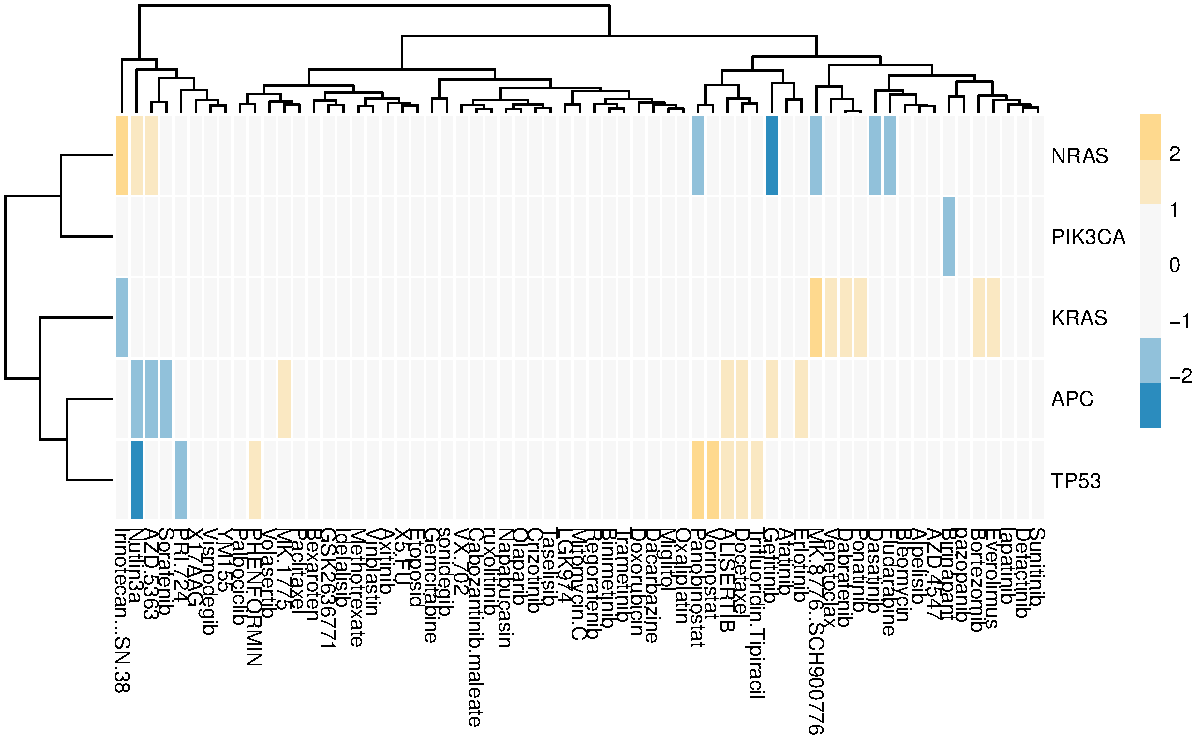
\includegraphics{organoid_unsupervised_exploration_files/figure-latex/unnamed-chunk-26-1.pdf}

\begin{Shaded}
\begin{Highlighting}[]
\NormalTok{umap_df }\OperatorTok
\StringTok{  }\KeywordTok{filter}\NormalTok{(drug }\OperatorTok{==}\StringTok{ "DMSO"}\NormalTok{) }\OperatorTok
\StringTok{  }\CommentTok{#sample_n(10000) %>%}
\StringTok{  }\KeywordTok{ggplot}\NormalTok{(}\KeywordTok{aes}\NormalTok{(v1, v2, }\DataTypeTok{color =}\NormalTok{ actin)) }\OperatorTok{+}\StringTok{ }
\StringTok{  }\KeywordTok{geom_point_rast}\NormalTok{(}\DataTypeTok{alpha =} \FloatTok{0.75}\NormalTok{, }\DataTypeTok{size =} \FloatTok{0.35}\NormalTok{) }\OperatorTok{+}
\StringTok{   }\KeywordTok{scale_colour_gradient}\NormalTok{(}\DataTypeTok{low =} \StringTok{"white"}\NormalTok{, }\DataTypeTok{high =} \StringTok{"red"}\NormalTok{) }\OperatorTok{+}\StringTok{ }
\StringTok{  }\KeywordTok{theme_cowplot}\NormalTok{() }\OperatorTok{+}
\StringTok{  }\KeywordTok{labs}\NormalTok{(}\DataTypeTok{x =} \StringTok{"UMAP 1"}\NormalTok{,}
       \DataTypeTok{y =} \StringTok{"UMAP 2"}\NormalTok{,}
       \DataTypeTok{title =} \StringTok{"Actin staining intensity"}\NormalTok{) }\OperatorTok{+}\StringTok{ }
\StringTok{  }\KeywordTok{theme}\NormalTok{(}\DataTypeTok{legend.position =} \StringTok{"bottom"}\NormalTok{) }\OperatorTok{+}\StringTok{ }
\StringTok{  }\KeywordTok{ggsave}\NormalTok{(}\KeywordTok{paste0}\NormalTok{(PATH, }\StringTok{"reports/figures/imaging/gg_actin.pdf"}\NormalTok{), }\DataTypeTok{width =} \DecValTok{4}\NormalTok{, }\DataTypeTok{height =} \DecValTok{4}\NormalTok{)}
\end{Highlighting}
\end{Shaded}

\includegraphics{organoid_unsupervised_exploration_files/figure-latex/unnamed-chunk-26-2.pdf}

\begin{Shaded}
\begin{Highlighting}[]
\NormalTok{umap_df }\OperatorTok
\StringTok{  }\KeywordTok{filter}\NormalTok{(drug }\OperatorTok{==}\StringTok{ "DMSO"}\NormalTok{) }\OperatorTok
\StringTok{  }\CommentTok{#sample_n(10000) %>%}
\StringTok{  }\KeywordTok{ggplot}\NormalTok{(}\KeywordTok{aes}\NormalTok{(v1, v2, }\DataTypeTok{color =}\NormalTok{ dapi)) }\OperatorTok{+}\StringTok{ }
\StringTok{  }\KeywordTok{geom_point_rast}\NormalTok{(}\DataTypeTok{alpha =} \FloatTok{0.75}\NormalTok{, }\DataTypeTok{size =} \FloatTok{0.35}\NormalTok{) }\OperatorTok{+}
\StringTok{   }\KeywordTok{scale_colour_gradient}\NormalTok{(}\DataTypeTok{low =} \StringTok{"white"}\NormalTok{, }\DataTypeTok{high =} \StringTok{"blue"}\NormalTok{) }\OperatorTok{+}\StringTok{ }
\StringTok{  }\KeywordTok{theme_cowplot}\NormalTok{() }\OperatorTok{+}
\StringTok{  }\KeywordTok{labs}\NormalTok{(}\DataTypeTok{x =} \StringTok{"UMAP 1"}\NormalTok{,}
       \DataTypeTok{y =} \StringTok{"UMAP 2"}\NormalTok{,}
       \DataTypeTok{title =} \StringTok{"DNA staining intensity"}\NormalTok{) }\OperatorTok{+}\StringTok{ }
\StringTok{  }\KeywordTok{theme}\NormalTok{(}\DataTypeTok{legend.position =} \StringTok{"bottom"}\NormalTok{) }\OperatorTok{+}\StringTok{ }
\StringTok{  }\KeywordTok{ggsave}\NormalTok{(}\KeywordTok{paste0}\NormalTok{(PATH, }\StringTok{"reports/figures/imaging/gg_dapi.pdf"}\NormalTok{), }\DataTypeTok{width =} \DecValTok{4}\NormalTok{, }\DataTypeTok{height =} \DecValTok{4}\NormalTok{)}
\end{Highlighting}
\end{Shaded}

\includegraphics{organoid_unsupervised_exploration_files/figure-latex/unnamed-chunk-26-3.pdf}

I am focusing on cystic vs solid organoid lines

\begin{Shaded}
\begin{Highlighting}[]
\CommentTok{#UMAP Cystic (Lines 18, 13, 27, 30) vs. Solid (others) treated with DMSO, for Figure 1 / matching expression analysis done for cystic vs. rest}

\KeywordTok{set.seed}\NormalTok{(}\DecValTok{123}\NormalTok{)}

\NormalTok{cystic_l <-}\StringTok{ }\NormalTok{organoid_morphology }\OperatorTok\StringTok{ }\KeywordTok{filter}\NormalTok{(morphology }\OperatorTok{==}\StringTok{ "cystic"}\NormalTok{) }\OperatorTok\NormalTok{.}\OperatorTok{$}\NormalTok{line }\OperatorTok\StringTok{ }\KeywordTok{paste0}\NormalTok{(., }\StringTok{"01"}\NormalTok{)}
\NormalTok{dense_l <-}\StringTok{ }\NormalTok{organoid_morphology }\OperatorTok\StringTok{ }\KeywordTok{filter}\NormalTok{(morphology }\OperatorTok{==}\StringTok{ "solid"}\NormalTok{) }\OperatorTok\NormalTok{.}\OperatorTok{$}\NormalTok{line }\OperatorTok\StringTok{ }\KeywordTok{paste0}\NormalTok{(., }\StringTok{"01"}\NormalTok{)}

\NormalTok{df <-}\StringTok{ }\NormalTok{umap_df }\OperatorTok
\StringTok{  }\KeywordTok{filter}\NormalTok{(drug }\OperatorTok{==}\StringTok{ "DMSO"}\NormalTok{) }\OperatorTok\StringTok{ }
\StringTok{  }\KeywordTok{filter}\NormalTok{(partition }\OperatorTok\StringTok{ }\KeywordTok{c}\NormalTok{(}\DecValTok{1}\NormalTok{,}\DecValTok{2}\NormalTok{)) }\OperatorTok
\StringTok{  }\KeywordTok{mutate}\NormalTok{(}\DataTypeTok{morphology =} \KeywordTok{case_when}\NormalTok{(line }\OperatorTok\StringTok{ }\NormalTok{cystic_l }\OperatorTok{~}\StringTok{ "cystic"}\NormalTok{,}
\NormalTok{                                line }\OperatorTok\StringTok{ }\NormalTok{dense_l }\OperatorTok{~}\StringTok{ "solid"}\NormalTok{,}
                                 \OtherTok{TRUE} \OperatorTok{~}\StringTok{ "other"}\NormalTok{))}

\NormalTok{gg_cystic <-}\StringTok{ }\NormalTok{umap_df }\OperatorTok\StringTok{ }
\StringTok{  }\KeywordTok{ggplot}\NormalTok{(}\KeywordTok{aes}\NormalTok{(v1, v2)) }\OperatorTok{+}\StringTok{ }
\StringTok{  }\KeywordTok{geom_point_rast}\NormalTok{(}\DataTypeTok{alpha =} \DecValTok{1}\NormalTok{, }\DataTypeTok{size =} \FloatTok{0.35}\NormalTok{, }\DataTypeTok{color =} \StringTok{"#f1f1f1"}\NormalTok{) }\OperatorTok{+}\StringTok{ }
\StringTok{  }
\StringTok{  }\CommentTok{# geom_point_rast(data = df %>%}
\StringTok{  }\CommentTok{#   filter(morphology == "cystic") %>% }
\StringTok{  }\CommentTok{#     sample_frac(0.05),}
\StringTok{  }\CommentTok{# aes(color = morphology),alpha = .4, size = 0.35, shape=16) + }
\StringTok{  }
\StringTok{  }\KeywordTok{geom_density_2d}\NormalTok{(}\DataTypeTok{data =}\NormalTok{ df }\OperatorTok\StringTok{ }\CommentTok{#geom_density_2d_filled}
\StringTok{    }\KeywordTok{filter}\NormalTok{(morphology }\OperatorTok{!=}\StringTok{ "other"}\NormalTok{), }\CommentTok{# %>% }
    \CommentTok{#  sample_frac(0.05)}
    \KeywordTok{aes}\NormalTok{(}\DataTypeTok{fill =}\NormalTok{ morphology), }\DataTypeTok{size =} \FloatTok{1.5}\NormalTok{) }\OperatorTok{+}

\StringTok{  }\CommentTok{#scale_color_brewer(type = "qual", palette = "Set2") +}
\StringTok{  }\CommentTok{#scale_fill_manual(values = c("#0571b0", "#ca0020")) +    }
\StringTok{  }\KeywordTok{scale_color_manual}\NormalTok{(}\DataTypeTok{values =} \KeywordTok{c}\NormalTok{(}\StringTok{"#0571b0"}\NormalTok{, }\StringTok{"#ca0020"}\NormalTok{)) }\OperatorTok{+}\StringTok{    }
\StringTok{  }\CommentTok{#geom_density2d(color = "black") + }
\StringTok{  }\KeywordTok{theme_classic}\NormalTok{() }\OperatorTok{+}
\StringTok{  }\KeywordTok{labs}\NormalTok{(}\DataTypeTok{x =} \StringTok{"UMAP 1"}\NormalTok{,}
       \DataTypeTok{y =} \StringTok{"UMAP 2"}\NormalTok{)}\OperatorTok{+}
\StringTok{       }\CommentTok{#caption = "control treated organoids") + }
\StringTok{  }\KeywordTok{theme_cowplot}\NormalTok{(}\DataTypeTok{font_size =} \DecValTok{8}\NormalTok{) }\OperatorTok{+}\StringTok{ }
\StringTok{  }\CommentTok{#theme(legend.position = "nothing")  + }
\StringTok{  }\KeywordTok{coord_fixed}\NormalTok{() }\OperatorTok{+}\StringTok{ }
\StringTok{  }\KeywordTok{scale_x_reverse}\NormalTok{()}


\NormalTok{gg_cystic}
\end{Highlighting}
\end{Shaded}

\hypertarget{plot-export}{%
\section{Plot Export}\label{plot-export}}

\begin{Shaded}
\begin{Highlighting}[]
\KeywordTok{plot_grid}\NormalTok{(}\KeywordTok{plot_grid}\NormalTok{(gg_size_dist_morph_ridge, gg_size_replicate, }\DataTypeTok{labels =} \KeywordTok{c}\NormalTok{(}\StringTok{'A'}\NormalTok{, }\StringTok{'B'}\NormalTok{), }\DataTypeTok{label_size =} \DecValTok{12}\NormalTok{, }\DataTypeTok{ncol =} \DecValTok{2}\NormalTok{),}
\NormalTok{          gg_size,}
          \KeywordTok{plot_grid}\NormalTok{(gg_line, gg_cystic, }\DataTypeTok{labels =} \KeywordTok{c}\NormalTok{(}\StringTok{'D'}\NormalTok{, }\StringTok{'E'}\NormalTok{), }\DataTypeTok{label_size =} \DecValTok{12}\NormalTok{, }\DataTypeTok{ncol =} \DecValTok{2}\NormalTok{),}
          \DataTypeTok{labels =} \KeywordTok{c}\NormalTok{(}\StringTok{''}\NormalTok{, }\StringTok{'C'}\NormalTok{, }\StringTok{''}\NormalTok{), }\DataTypeTok{label_size =} \DecValTok{12}\NormalTok{, }\DataTypeTok{ncol =} \DecValTok{1}\NormalTok{) }\OperatorTok{+}
\StringTok{  }\KeywordTok{ggsave}\NormalTok{(}\KeywordTok{paste0}\NormalTok{(PATH, }\StringTok{"reports/panels/imaging/panel_size_dist.pdf"}\NormalTok{), }\DataTypeTok{width =} \DecValTok{8}\NormalTok{, }\DataTypeTok{height =} \DecValTok{16}\NormalTok{)}

\KeywordTok{plot_grid}\NormalTok{(}\KeywordTok{plot_grid}\NormalTok{(ggdrug_size, ggdrug_count, }\DataTypeTok{labels =} \KeywordTok{c}\NormalTok{(}\StringTok{'A'}\NormalTok{, }\StringTok{'B'}\NormalTok{), }\DataTypeTok{label_size =} \DecValTok{12}\NormalTok{),}
\NormalTok{          gg_drug,}
\NormalTok{          gg_size_drug,}
          \DataTypeTok{labels =} \KeywordTok{c}\NormalTok{(}\StringTok{''}\NormalTok{, }\StringTok{'C'}\NormalTok{, }\StringTok{'D'}\NormalTok{), }\DataTypeTok{label_size =} \DecValTok{12}\NormalTok{, }\DataTypeTok{ncol =} \DecValTok{1}\NormalTok{) }\OperatorTok{+}
\StringTok{  }\KeywordTok{ggsave}\NormalTok{(}\KeywordTok{paste0}\NormalTok{(PATH, }\StringTok{"reports/panels/imaging/panel_size_drug.pdf"}\NormalTok{), }\DataTypeTok{width =} \DecValTok{8}\NormalTok{, }\DataTypeTok{height =} \DecValTok{12}\NormalTok{)}

\NormalTok{gg_size_supp}
\end{Highlighting}
\end{Shaded}

\begin{Shaded}
\begin{Highlighting}[]
\KeywordTok{sessionInfo}\NormalTok{()}
\end{Highlighting}
\end{Shaded}

\begin{verbatim}
## R version 4.0.0 (2020-04-24)
## Platform: x86_64-pc-linux-gnu (64-bit)
## Running under: Ubuntu 20.04.2 LTS
## 
## Matrix products: default
## BLAS/LAPACK: /usr/lib/x86_64-linux-gnu/openblas-pthread/libopenblasp-r0.3.8.so
## 
## locale:
##  [1] LC_CTYPE=en_US.UTF-8       LC_NUMERIC=C              
##  [3] LC_TIME=en_US.UTF-8        LC_COLLATE=en_US.UTF-8    
##  [5] LC_MONETARY=en_US.UTF-8    LC_MESSAGES=C             
##  [7] LC_PAPER=en_US.UTF-8       LC_NAME=C                 
##  [9] LC_ADDRESS=C               LC_TELEPHONE=C            
## [11] LC_MEASUREMENT=en_US.UTF-8 LC_IDENTIFICATION=C       
## 
## attached base packages:
## [1] stats     graphics  grDevices utils     datasets  methods   base     
## 
## other attached packages:
##  [1] ggridges_0.5.2  scico_1.1.0     princurve_2.1.4 cowplot_1.0.0  
##  [5] ggrastr_0.2.3   here_0.1        readr_1.3.1     purrr_0.3.4    
##  [9] magrittr_1.5    tidyr_1.1.0     dplyr_1.0.0     ggplot2_3.3.1  
## 
## loaded via a namespace (and not attached):
##  [1] beeswarm_0.2.3     tidyselect_1.1.0   xfun_0.14          splines_4.0.0     
##  [5] lattice_0.20-41    colorspace_1.4-1   vctrs_0.3.1        generics_0.0.2    
##  [9] viridisLite_0.3.0  htmltools_0.4.0    mgcv_1.8-31        yaml_2.2.1        
## [13] utf8_1.1.4         survival_3.1-12    rlang_0.4.6        pillar_1.4.4      
## [17] glue_1.4.1         withr_2.2.0        fitdistrplus_1.1-1 RColorBrewer_1.1-2
## [21] lifecycle_0.2.0    plyr_1.8.6         stringr_1.4.0      munsell_0.5.0     
## [25] gtable_0.3.0       evaluate_0.14      labeling_0.3       knitr_1.28        
## [29] Cairo_1.5-12       vipor_0.4.5        fansi_0.4.1        broom_0.5.6       
## [33] Rcpp_1.0.4.6       scales_1.1.1       backports_1.1.7    farver_2.0.3      
## [37] hms_0.5.3          digest_0.6.25      stringi_1.4.6      ggrepel_0.8.2     
## [41] grid_4.0.0         rprojroot_1.3-2    cli_2.0.2          tools_4.0.0       
## [45] tibble_3.0.1       crayon_1.3.4       pkgconfig_2.0.3    MASS_7.3-51.5     
## [49] ellipsis_0.3.1     Matrix_1.2-18      ggbeeswarm_0.6.0   assertthat_0.2.1  
## [53] rmarkdown_2.2      R6_2.4.1           nlme_3.1-147       compiler_4.0.0
\end{verbatim}

\end{document}
